% Generated by Sphinx.
\def\sphinxdocclass{report}
\documentclass[a4paper,12pt,spanish]{sphinxmanual}
\usepackage[utf8]{inputenc}
\DeclareUnicodeCharacter{00A0}{\nobreakspace}
\usepackage{cmap}
\usepackage[T1]{fontenc}
\usepackage{babel}
\usepackage{times}
\usepackage[Sonny]{fncychap}
\usepackage{longtable}
\usepackage{sphinx}
\usepackage{multirow}


\title{Programación de Servicios y Procesos}
\date{30 de October de 2014}
\release{1.0}
\author{Oscar Gomez}
\newcommand{\sphinxlogo}{}
\renewcommand{\releasename}{Publicación}
\makeindex

\makeatletter
\def\PYG@reset{\let\PYG@it=\relax \let\PYG@bf=\relax%
    \let\PYG@ul=\relax \let\PYG@tc=\relax%
    \let\PYG@bc=\relax \let\PYG@ff=\relax}
\def\PYG@tok#1{\csname PYG@tok@#1\endcsname}
\def\PYG@toks#1+{\ifx\relax#1\empty\else%
    \PYG@tok{#1}\expandafter\PYG@toks\fi}
\def\PYG@do#1{\PYG@bc{\PYG@tc{\PYG@ul{%
    \PYG@it{\PYG@bf{\PYG@ff{#1}}}}}}}
\def\PYG#1#2{\PYG@reset\PYG@toks#1+\relax+\PYG@do{#2}}

\expandafter\def\csname PYG@tok@o\endcsname{\def\PYG@tc##1{\textcolor[rgb]{0.40,0.40,0.40}{##1}}}
\expandafter\def\csname PYG@tok@mh\endcsname{\def\PYG@tc##1{\textcolor[rgb]{0.13,0.50,0.31}{##1}}}
\expandafter\def\csname PYG@tok@mo\endcsname{\def\PYG@tc##1{\textcolor[rgb]{0.13,0.50,0.31}{##1}}}
\expandafter\def\csname PYG@tok@nd\endcsname{\let\PYG@bf=\textbf\def\PYG@tc##1{\textcolor[rgb]{0.33,0.33,0.33}{##1}}}
\expandafter\def\csname PYG@tok@il\endcsname{\def\PYG@tc##1{\textcolor[rgb]{0.13,0.50,0.31}{##1}}}
\expandafter\def\csname PYG@tok@go\endcsname{\def\PYG@tc##1{\textcolor[rgb]{0.20,0.20,0.20}{##1}}}
\expandafter\def\csname PYG@tok@no\endcsname{\def\PYG@tc##1{\textcolor[rgb]{0.38,0.68,0.84}{##1}}}
\expandafter\def\csname PYG@tok@kr\endcsname{\let\PYG@bf=\textbf\def\PYG@tc##1{\textcolor[rgb]{0.00,0.44,0.13}{##1}}}
\expandafter\def\csname PYG@tok@c1\endcsname{\let\PYG@it=\textit\def\PYG@tc##1{\textcolor[rgb]{0.25,0.50,0.56}{##1}}}
\expandafter\def\csname PYG@tok@nc\endcsname{\let\PYG@bf=\textbf\def\PYG@tc##1{\textcolor[rgb]{0.05,0.52,0.71}{##1}}}
\expandafter\def\csname PYG@tok@kp\endcsname{\def\PYG@tc##1{\textcolor[rgb]{0.00,0.44,0.13}{##1}}}
\expandafter\def\csname PYG@tok@nv\endcsname{\def\PYG@tc##1{\textcolor[rgb]{0.73,0.38,0.84}{##1}}}
\expandafter\def\csname PYG@tok@vg\endcsname{\def\PYG@tc##1{\textcolor[rgb]{0.73,0.38,0.84}{##1}}}
\expandafter\def\csname PYG@tok@vc\endcsname{\def\PYG@tc##1{\textcolor[rgb]{0.73,0.38,0.84}{##1}}}
\expandafter\def\csname PYG@tok@ne\endcsname{\def\PYG@tc##1{\textcolor[rgb]{0.00,0.44,0.13}{##1}}}
\expandafter\def\csname PYG@tok@gs\endcsname{\let\PYG@bf=\textbf}
\expandafter\def\csname PYG@tok@gt\endcsname{\def\PYG@tc##1{\textcolor[rgb]{0.00,0.27,0.87}{##1}}}
\expandafter\def\csname PYG@tok@mf\endcsname{\def\PYG@tc##1{\textcolor[rgb]{0.13,0.50,0.31}{##1}}}
\expandafter\def\csname PYG@tok@si\endcsname{\let\PYG@it=\textit\def\PYG@tc##1{\textcolor[rgb]{0.44,0.63,0.82}{##1}}}
\expandafter\def\csname PYG@tok@gp\endcsname{\let\PYG@bf=\textbf\def\PYG@tc##1{\textcolor[rgb]{0.78,0.36,0.04}{##1}}}
\expandafter\def\csname PYG@tok@sc\endcsname{\def\PYG@tc##1{\textcolor[rgb]{0.25,0.44,0.63}{##1}}}
\expandafter\def\csname PYG@tok@cs\endcsname{\def\PYG@tc##1{\textcolor[rgb]{0.25,0.50,0.56}{##1}}\def\PYG@bc##1{\setlength{\fboxsep}{0pt}\colorbox[rgb]{1.00,0.94,0.94}{\strut ##1}}}
\expandafter\def\csname PYG@tok@kc\endcsname{\let\PYG@bf=\textbf\def\PYG@tc##1{\textcolor[rgb]{0.00,0.44,0.13}{##1}}}
\expandafter\def\csname PYG@tok@vi\endcsname{\def\PYG@tc##1{\textcolor[rgb]{0.73,0.38,0.84}{##1}}}
\expandafter\def\csname PYG@tok@gd\endcsname{\def\PYG@tc##1{\textcolor[rgb]{0.63,0.00,0.00}{##1}}}
\expandafter\def\csname PYG@tok@cp\endcsname{\def\PYG@tc##1{\textcolor[rgb]{0.00,0.44,0.13}{##1}}}
\expandafter\def\csname PYG@tok@bp\endcsname{\def\PYG@tc##1{\textcolor[rgb]{0.00,0.44,0.13}{##1}}}
\expandafter\def\csname PYG@tok@gu\endcsname{\let\PYG@bf=\textbf\def\PYG@tc##1{\textcolor[rgb]{0.50,0.00,0.50}{##1}}}
\expandafter\def\csname PYG@tok@nf\endcsname{\def\PYG@tc##1{\textcolor[rgb]{0.02,0.16,0.49}{##1}}}
\expandafter\def\csname PYG@tok@c\endcsname{\let\PYG@it=\textit\def\PYG@tc##1{\textcolor[rgb]{0.25,0.50,0.56}{##1}}}
\expandafter\def\csname PYG@tok@s1\endcsname{\def\PYG@tc##1{\textcolor[rgb]{0.25,0.44,0.63}{##1}}}
\expandafter\def\csname PYG@tok@err\endcsname{\def\PYG@bc##1{\setlength{\fboxsep}{0pt}\fcolorbox[rgb]{1.00,0.00,0.00}{1,1,1}{\strut ##1}}}
\expandafter\def\csname PYG@tok@se\endcsname{\let\PYG@bf=\textbf\def\PYG@tc##1{\textcolor[rgb]{0.25,0.44,0.63}{##1}}}
\expandafter\def\csname PYG@tok@s\endcsname{\def\PYG@tc##1{\textcolor[rgb]{0.25,0.44,0.63}{##1}}}
\expandafter\def\csname PYG@tok@gh\endcsname{\let\PYG@bf=\textbf\def\PYG@tc##1{\textcolor[rgb]{0.00,0.00,0.50}{##1}}}
\expandafter\def\csname PYG@tok@nl\endcsname{\let\PYG@bf=\textbf\def\PYG@tc##1{\textcolor[rgb]{0.00,0.13,0.44}{##1}}}
\expandafter\def\csname PYG@tok@kn\endcsname{\let\PYG@bf=\textbf\def\PYG@tc##1{\textcolor[rgb]{0.00,0.44,0.13}{##1}}}
\expandafter\def\csname PYG@tok@sx\endcsname{\def\PYG@tc##1{\textcolor[rgb]{0.78,0.36,0.04}{##1}}}
\expandafter\def\csname PYG@tok@gr\endcsname{\def\PYG@tc##1{\textcolor[rgb]{1.00,0.00,0.00}{##1}}}
\expandafter\def\csname PYG@tok@sb\endcsname{\def\PYG@tc##1{\textcolor[rgb]{0.25,0.44,0.63}{##1}}}
\expandafter\def\csname PYG@tok@k\endcsname{\let\PYG@bf=\textbf\def\PYG@tc##1{\textcolor[rgb]{0.00,0.44,0.13}{##1}}}
\expandafter\def\csname PYG@tok@m\endcsname{\def\PYG@tc##1{\textcolor[rgb]{0.13,0.50,0.31}{##1}}}
\expandafter\def\csname PYG@tok@gi\endcsname{\def\PYG@tc##1{\textcolor[rgb]{0.00,0.63,0.00}{##1}}}
\expandafter\def\csname PYG@tok@sr\endcsname{\def\PYG@tc##1{\textcolor[rgb]{0.14,0.33,0.53}{##1}}}
\expandafter\def\csname PYG@tok@kt\endcsname{\def\PYG@tc##1{\textcolor[rgb]{0.56,0.13,0.00}{##1}}}
\expandafter\def\csname PYG@tok@s2\endcsname{\def\PYG@tc##1{\textcolor[rgb]{0.25,0.44,0.63}{##1}}}
\expandafter\def\csname PYG@tok@sh\endcsname{\def\PYG@tc##1{\textcolor[rgb]{0.25,0.44,0.63}{##1}}}
\expandafter\def\csname PYG@tok@nt\endcsname{\let\PYG@bf=\textbf\def\PYG@tc##1{\textcolor[rgb]{0.02,0.16,0.45}{##1}}}
\expandafter\def\csname PYG@tok@nb\endcsname{\def\PYG@tc##1{\textcolor[rgb]{0.00,0.44,0.13}{##1}}}
\expandafter\def\csname PYG@tok@nn\endcsname{\let\PYG@bf=\textbf\def\PYG@tc##1{\textcolor[rgb]{0.05,0.52,0.71}{##1}}}
\expandafter\def\csname PYG@tok@ow\endcsname{\let\PYG@bf=\textbf\def\PYG@tc##1{\textcolor[rgb]{0.00,0.44,0.13}{##1}}}
\expandafter\def\csname PYG@tok@cm\endcsname{\let\PYG@it=\textit\def\PYG@tc##1{\textcolor[rgb]{0.25,0.50,0.56}{##1}}}
\expandafter\def\csname PYG@tok@ge\endcsname{\let\PYG@it=\textit}
\expandafter\def\csname PYG@tok@sd\endcsname{\let\PYG@it=\textit\def\PYG@tc##1{\textcolor[rgb]{0.25,0.44,0.63}{##1}}}
\expandafter\def\csname PYG@tok@ni\endcsname{\let\PYG@bf=\textbf\def\PYG@tc##1{\textcolor[rgb]{0.84,0.33,0.22}{##1}}}
\expandafter\def\csname PYG@tok@ss\endcsname{\def\PYG@tc##1{\textcolor[rgb]{0.32,0.47,0.09}{##1}}}
\expandafter\def\csname PYG@tok@w\endcsname{\def\PYG@tc##1{\textcolor[rgb]{0.73,0.73,0.73}{##1}}}
\expandafter\def\csname PYG@tok@kd\endcsname{\let\PYG@bf=\textbf\def\PYG@tc##1{\textcolor[rgb]{0.00,0.44,0.13}{##1}}}
\expandafter\def\csname PYG@tok@na\endcsname{\def\PYG@tc##1{\textcolor[rgb]{0.25,0.44,0.63}{##1}}}
\expandafter\def\csname PYG@tok@mi\endcsname{\def\PYG@tc##1{\textcolor[rgb]{0.13,0.50,0.31}{##1}}}

\def\PYGZbs{\char`\\}
\def\PYGZus{\char`\_}
\def\PYGZob{\char`\{}
\def\PYGZcb{\char`\}}
\def\PYGZca{\char`\^}
\def\PYGZam{\char`\&}
\def\PYGZlt{\char`\<}
\def\PYGZgt{\char`\>}
\def\PYGZsh{\char`\#}
\def\PYGZpc{\char`\%}
\def\PYGZdl{\char`\$}
\def\PYGZhy{\char`\-}
\def\PYGZsq{\char`\'}
\def\PYGZdq{\char`\"}
\def\PYGZti{\char`\~}
% for compatibility with earlier versions
\def\PYGZat{@}
\def\PYGZlb{[}
\def\PYGZrb{]}
\makeatother

\renewcommand\PYGZsq{\textquotesingle}

\begin{document}
\shorthandoff{"}
\maketitle
\tableofcontents
\phantomsection\label{index::doc}



\chapter{Programación multiproceso}
\label{textos/tema1:programacion-multiproceso}\label{textos/tema1:programacion-de-servicios-y-procesos}\label{textos/tema1::doc}

\section{Ejecutables. Procesos. Servicios.}
\label{textos/tema1:ejecutables-procesos-servicios}

\subsection{Ejecutables}
\label{textos/tema1:ejecutables}
Un ejecutable es un archivo con la estructura necesaria para que el sistema operativo pueda poner en marcha el programa que hay dentro. En Windows, los ejecutables suelen ser archivos con la extension .EXE.

Sin embargo, Java genera ficheros .JAR o .CLASS. Estos ficheros \emph{no son ejecutables} sino que son archivos que el intérprete de JAVA (el archivo \code{java.exe}) leerá y ejecutará.

El intérprete toma el programa y lo traduce a instrucciones del microprocesador en el que estemos, que puede ser x86 o un x64 o lo que sea. Ese proceso se hace ``al instante'' o JIT (Just-In-Time).

Un EXE puede que no contenga las instrucciones de los microprocesadores más modernos. Como todos son compatibles no es un gran problema, sin embargo, puede que no aprovechemos al 100\% la capacidad de nuestro micro.


\subsection{Procesos}
\label{textos/tema1:procesos}
Es un archivo que está en ejecución y bajo el control del sistema operativo. Un proceso puede atravesar diversas etapas en su ``ciclo de vida''. Los estados en los que puede estar son:
\begin{itemize}
\item {} 
En ejecución: está dentro del microprocesador.

\item {} 
Pausado/detenido/en espera: el proceso tiene que seguir en ejecución pero en ese momento el S.O tomó la decisión de dejar paso a otro.

\item {} 
Interrumpido: el proceso tiene que seguir en ejecución pero \emph{el usuario} ha decidido interrumpir la ejecución.

\item {} 
Existen otros estados pero ya son muy dependientes del sistema operativo concreto.

\end{itemize}


\subsection{Servicios}
\label{textos/tema1:servicios}
Un servicio es un proceso que no muestra ninguna ventana ni gráfico en pantalla porque no está pensado para que el usuario lo maneje directamente.

Habitualmente, un servicio es un programa que atiende a otro programa.


\section{Hilos.}
\label{textos/tema1:hilos}
Un hilo es un concepto más avanzado que un proceso: al hablar de procesos cada uno tiene su propio espacio en memoria. Si abrimos 20 procesos cada uno de ellos consume 20x de memoria RAM. Un hilo es un proceso mucho más ligero, en el que el código y los datos se comparten de una forma distinta.

Un proceso no tiene acceso a los datos de otro procesos. Sin embargo un hilo sí accede a los datos de otro hilo. Esto complicará algunas cuestiones a la hora de programar.


\section{Programación concurrente.}
\label{textos/tema1:programacion-concurrente}
La programación concurrente es la parte de la programación que se ocupa de crear programas que pueden tener varios procesos/hilos que colaboran para ejecutar un trabajo y aprovechar al máximo el rendimiento de sistemas multinúcleo.


\section{Programación paralela y distribuida.}
\label{textos/tema1:programacion-paralela-y-distribuida}
Dentro de la programación concurrente tenemos la paralela y la distribuida:
\begin{itemize}
\item {} 
En general se denomina ``programación paralela'' a la creación de software que se ejecuta siempre en un solo ordenador (con varios núcleos o no)

\item {} 
Se denomina ``programación distribuida'' a la creación de software que se ejecuta en ordenadores distintos y que se comunican a través de una red.

\end{itemize}


\section{Creación de procesos.}
\label{textos/tema1:creacion-de-procesos}
En Java es posible crear procesos utilizando algunas clases que el entorno ofrece para esta tarea. En este tema, veremos en profundidad la clase ProcessBuilder.

El ejemplo siguiente muestra como lanzar un proceso de Acrobat Reader:

\begin{Verbatim}[commandchars=\\\{\}]
\PYG{k+kd}{public} \PYG{k+kd}{class} \PYG{n+nc}{LanzadorProcesos} \PYG{o}{\PYGZob{}}
        \PYG{k+kd}{public} \PYG{k+kt}{void} \PYG{n+nf}{ejecutar}\PYG{o}{(}\PYG{n}{String} \PYG{n}{ruta}\PYG{o}{)}\PYG{o}{\PYGZob{}}

                \PYG{n}{ProcessBuilder} \PYG{n}{pb}\PYG{o}{;}
                \PYG{k}{try} \PYG{o}{\PYGZob{}}
                        \PYG{n}{pb} \PYG{o}{=} \PYG{k}{new} \PYG{n}{ProcessBuilder}\PYG{o}{(}\PYG{n}{ruta}\PYG{o}{)}\PYG{o}{;}
                        \PYG{n}{pb}\PYG{o}{.}\PYG{n+na}{start}\PYG{o}{(}\PYG{o}{)}\PYG{o}{;}
                \PYG{o}{\PYGZcb{}} \PYG{k}{catch} \PYG{o}{(}\PYG{n}{Exception} \PYG{n}{e}\PYG{o}{)} \PYG{o}{\PYGZob{}}
                        \PYG{c+c1}{// TODO Auto\PYGZhy{}generated catch block}
                        \PYG{n}{e}\PYG{o}{.}\PYG{n+na}{printStackTrace}\PYG{o}{(}\PYG{o}{)}\PYG{o}{;}
                \PYG{o}{\PYGZcb{}}

        \PYG{o}{\PYGZcb{}}
        \PYG{c+cm}{/**}
\PYG{c+cm}{         * @param args}
\PYG{c+cm}{         */}
        \PYG{k+kd}{public} \PYG{k+kd}{static} \PYG{k+kt}{void} \PYG{n+nf}{main}\PYG{o}{(}\PYG{n}{String}\PYG{o}{[}\PYG{o}{]} \PYG{n}{args}\PYG{o}{)} \PYG{o}{\PYGZob{}}
                \PYG{n}{String} \PYG{n}{ruta}\PYG{o}{=}
                        \PYG{l+s}{\PYGZdq{}C:\PYGZbs{}\PYGZbs{}Program Files (x86)\PYGZbs{}\PYGZbs{}Adobe\PYGZbs{}\PYGZbs{}Reader 11.0\PYGZbs{}\PYGZbs{}Reader\PYGZbs{}\PYGZbs{}AcroRd32.exe\PYGZdq{}}\PYG{o}{;}
                \PYG{n}{LanzadorProcesos} \PYG{n}{lp}\PYG{o}{=}\PYG{k}{new} \PYG{n}{LanzadorProcesos}\PYG{o}{(}\PYG{o}{)}\PYG{o}{;}
                \PYG{n}{lp}\PYG{o}{.}\PYG{n+na}{ejecutar}\PYG{o}{(}\PYG{n}{ruta}\PYG{o}{)}\PYG{o}{;}
                \PYG{n}{System}\PYG{o}{.}\PYG{n+na}{out}\PYG{o}{.}\PYG{n+na}{println}\PYG{o}{(}\PYG{l+s}{\PYGZdq{}Finalizado\PYGZdq{}}\PYG{o}{)}\PYG{o}{;}
        \PYG{o}{\PYGZcb{}}

\PYG{o}{\PYGZcb{}}
\end{Verbatim}

Supongamos que necesitamos crear un programa que aproveche al máximo el número de CPUs para realizar alguna tarea intensiva. Supongamos que dicha tarea consiste en sumar números.

Enunciado: crear una clase Java que sea capaz de sumar todos los números comprendidos entre dos valores incluyendo ambos valores.

Para resolverlo crearemos una clase \code{Sumador} que tenga un método que acepte dos números \code{n1} y \code{n2} y que devuelva la suma de todo el intervalor.

Además, incluiremos un método \code{main} que ejecute la operación de suma tomando los números de la línea de comandos (es decir, se pasan como argumentos al main).

El código de dicha clase podría ser algo así:

\begin{Verbatim}[commandchars=\\\{\}]
\PYG{k+kn}{package} \PYG{n}{com}\PYG{o}{.}\PYG{n+na}{ies}\PYG{o}{;}

\PYG{k+kd}{public} \PYG{k+kd}{class} \PYG{n+nc}{Sumador} \PYG{o}{\PYGZob{}}
        \PYG{k+kd}{public} \PYG{k+kt}{int} \PYG{n+nf}{sumar}\PYG{o}{(}\PYG{k+kt}{int} \PYG{n}{n1}\PYG{o}{,} \PYG{k+kt}{int} \PYG{n}{n2}\PYG{o}{)}\PYG{o}{\PYGZob{}}
                \PYG{k+kt}{int} \PYG{n}{resultado}\PYG{o}{=}\PYG{l+m+mi}{0}\PYG{o}{;}
                \PYG{k}{for} \PYG{o}{(}\PYG{k+kt}{int} \PYG{n}{i}\PYG{o}{=}\PYG{n}{n1}\PYG{o}{;}\PYG{n}{i}\PYG{o}{\PYGZlt{}}\PYG{o}{=}\PYG{n}{n2}\PYG{o}{;}\PYG{n}{i}\PYG{o}{+}\PYG{o}{+}\PYG{o}{)}\PYG{o}{\PYGZob{}}
                        \PYG{n}{resultado}\PYG{o}{=}\PYG{n}{resultado}\PYG{o}{+}\PYG{n}{i}\PYG{o}{;}
                \PYG{o}{\PYGZcb{}}
                \PYG{k}{return} \PYG{n}{resultado}\PYG{o}{;}
        \PYG{o}{\PYGZcb{}}
        \PYG{k+kd}{public} \PYG{k+kd}{static} \PYG{k+kt}{void} \PYG{n+nf}{main}\PYG{o}{(}\PYG{n}{String}\PYG{o}{[}\PYG{o}{]} \PYG{n}{args}\PYG{o}{)}\PYG{o}{\PYGZob{}}
                \PYG{n}{Sumador} \PYG{n}{s}\PYG{o}{=}\PYG{k}{new} \PYG{n}{Sumador}\PYG{o}{(}\PYG{o}{)}\PYG{o}{;}
                \PYG{k+kt}{int} \PYG{n}{n1}\PYG{o}{=}\PYG{n}{Integer}\PYG{o}{.}\PYG{n+na}{parseInt}\PYG{o}{(}\PYG{n}{args}\PYG{o}{[}\PYG{l+m+mi}{0}\PYG{o}{]}\PYG{o}{)}\PYG{o}{;}
                \PYG{k+kt}{int} \PYG{n}{n2}\PYG{o}{=}\PYG{n}{Integer}\PYG{o}{.}\PYG{n+na}{parseInt}\PYG{o}{(}\PYG{n}{args}\PYG{o}{[}\PYG{l+m+mi}{1}\PYG{o}{]}\PYG{o}{)}\PYG{o}{;}
                \PYG{k+kt}{int} \PYG{n}{resultado}\PYG{o}{=}\PYG{n}{s}\PYG{o}{.}\PYG{n+na}{sumar}\PYG{o}{(}\PYG{n}{n1}\PYG{o}{,} \PYG{n}{n2}\PYG{o}{)}\PYG{o}{;}
                \PYG{n}{System}\PYG{o}{.}\PYG{n+na}{out}\PYG{o}{.}\PYG{n+na}{println}\PYG{o}{(}\PYG{n}{resultado}\PYG{o}{)}\PYG{o}{;}
        \PYG{o}{\PYGZcb{}}
\PYG{o}{\PYGZcb{}}
\end{Verbatim}

Para ejecutar este programa desde dentro de Eclipse es necesario indicar que deseamos enviar \emph{argumentos} al programa. Por ejemplo, si deseamos sumar los números del 2 al 10, deberemos ir a la venta ``Run configuration'' y en la pestaña ``Arguments'' indicar los argumentos (que en este caso son los dos números a indicar).
\begin{figure}[htbp]
\centering
\capstart

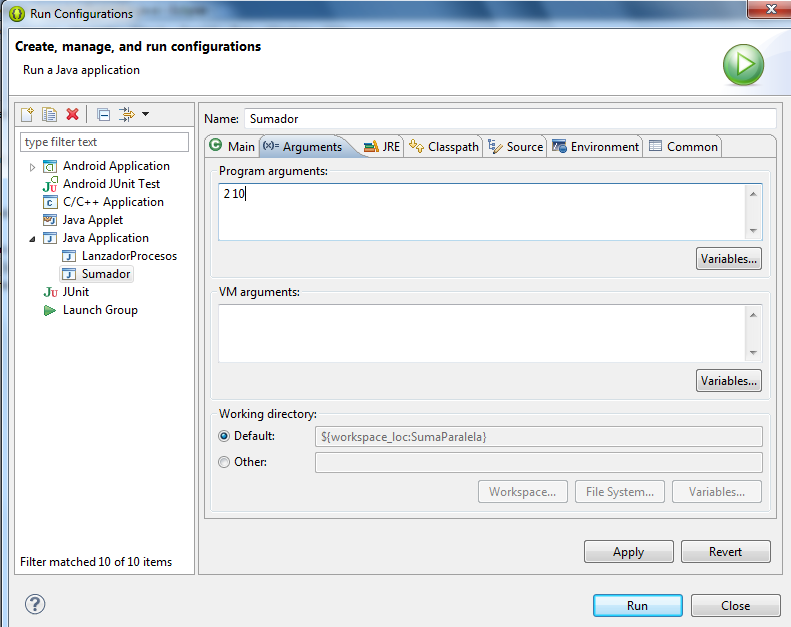
\includegraphics{configuraciones.png}
\caption{Modificando los argumentos del programa}\end{figure}

Una vez hecha la prueba de la clase sumador, le quitamos el main, y crearemos una clase que sea capaz de lanzar varios procesos. La clase \code{Sumador} se quedará así:

\begin{Verbatim}[commandchars=\\\{\}]
\PYG{k+kd}{public} \PYG{k+kd}{class} \PYG{n+nc}{Sumador} \PYG{o}{\PYGZob{}}
        \PYG{k+kd}{public} \PYG{k+kt}{int} \PYG{n+nf}{sumar}\PYG{o}{(}\PYG{k+kt}{int} \PYG{n}{n1}\PYG{o}{,} \PYG{k+kt}{int} \PYG{n}{n2}\PYG{o}{)}\PYG{o}{\PYGZob{}}
                \PYG{k+kt}{int} \PYG{n}{resultado}\PYG{o}{=}\PYG{l+m+mi}{0}\PYG{o}{;}
                \PYG{k}{for} \PYG{o}{(}\PYG{k+kt}{int} \PYG{n}{i}\PYG{o}{=}\PYG{n}{n1}\PYG{o}{;}\PYG{n}{i}\PYG{o}{\PYGZlt{}}\PYG{o}{=}\PYG{n}{n2}\PYG{o}{;}\PYG{n}{i}\PYG{o}{+}\PYG{o}{+}\PYG{o}{)}\PYG{o}{\PYGZob{}}
                        \PYG{n}{resultado}\PYG{o}{=}\PYG{n}{resultado}\PYG{o}{+}\PYG{n}{i}\PYG{o}{;}
                \PYG{o}{\PYGZcb{}}
                \PYG{k}{return} \PYG{n}{resultado}\PYG{o}{;}
        \PYG{o}{\PYGZcb{}}
\PYG{o}{\PYGZcb{}}
\end{Verbatim}

Y ahora tendremos una clase que lanza procesos de esta forma:

\begin{Verbatim}[commandchars=\\\{\}]
\PYG{k+kn}{package} \PYG{n}{com}\PYG{o}{.}\PYG{n+na}{ies}\PYG{o}{;}

\PYG{k+kd}{public} \PYG{k+kd}{class} \PYG{n+nc}{Lanzador} \PYG{o}{\PYGZob{}}
        \PYG{k+kd}{public} \PYG{k+kt}{void} \PYG{n+nf}{lanzarSumador}\PYG{o}{(}\PYG{n}{Integer} \PYG{n}{n1}\PYG{o}{,}
                        \PYG{n}{Integer} \PYG{n}{n2}\PYG{o}{)}\PYG{o}{\PYGZob{}}
                \PYG{n}{String} \PYG{n}{clase}\PYG{o}{=}\PYG{l+s}{\PYGZdq{}com.ies.Sumador\PYGZdq{}}\PYG{o}{;}
                \PYG{n}{ProcessBuilder} \PYG{n}{pb}\PYG{o}{;}
                \PYG{k}{try} \PYG{o}{\PYGZob{}}
                        \PYG{n}{pb} \PYG{o}{=} \PYG{k}{new} \PYG{n}{ProcessBuilder}\PYG{o}{(}
                                        \PYG{l+s}{\PYGZdq{}java\PYGZdq{}}\PYG{o}{,}\PYG{n}{clase}\PYG{o}{,}
                                        \PYG{n}{n1}\PYG{o}{.}\PYG{n+na}{toString}\PYG{o}{(}\PYG{o}{)}\PYG{o}{,}
                                        \PYG{n}{n2}\PYG{o}{.}\PYG{n+na}{toString}\PYG{o}{(}\PYG{o}{)}\PYG{o}{)}\PYG{o}{;}
                        \PYG{n}{pb}\PYG{o}{.}\PYG{n+na}{start}\PYG{o}{(}\PYG{o}{)}\PYG{o}{;}
                \PYG{o}{\PYGZcb{}} \PYG{k}{catch} \PYG{o}{(}\PYG{n}{Exception} \PYG{n}{e}\PYG{o}{)} \PYG{o}{\PYGZob{}}
                        \PYG{c+c1}{// TODO Auto\PYGZhy{}generated catch block}
                        \PYG{n}{e}\PYG{o}{.}\PYG{n+na}{printStackTrace}\PYG{o}{(}\PYG{o}{)}\PYG{o}{;}
                \PYG{o}{\PYGZcb{}}
        \PYG{o}{\PYGZcb{}}
        \PYG{k+kd}{public} \PYG{k+kd}{static} \PYG{k+kt}{void} \PYG{n+nf}{main}\PYG{o}{(}\PYG{n}{String}\PYG{o}{[}\PYG{o}{]} \PYG{n}{args}\PYG{o}{)}\PYG{o}{\PYGZob{}}
                \PYG{n}{Lanzador} \PYG{n}{l}\PYG{o}{=}\PYG{k}{new} \PYG{n}{Lanzador}\PYG{o}{(}\PYG{o}{)}\PYG{o}{;}
                \PYG{n}{l}\PYG{o}{.}\PYG{n+na}{lanzarSumador}\PYG{o}{(}\PYG{l+m+mi}{1}\PYG{o}{,} \PYG{l+m+mi}{51}\PYG{o}{)}\PYG{o}{;}
                \PYG{n}{l}\PYG{o}{.}\PYG{n+na}{lanzarSumador}\PYG{o}{(}\PYG{l+m+mi}{51}\PYG{o}{,} \PYG{l+m+mi}{100}\PYG{o}{)}\PYG{o}{;}
                \PYG{n}{System}\PYG{o}{.}\PYG{n+na}{out}\PYG{o}{.}\PYG{n+na}{println}\PYG{o}{(}\PYG{l+s}{\PYGZdq{}Ok\PYGZdq{}}\PYG{o}{)}\PYG{o}{;}
        \PYG{o}{\PYGZcb{}}
\PYG{o}{\PYGZcb{}}
\end{Verbatim}


\section{Comunicación entre procesos.}
\label{textos/tema1:comunicacion-entre-procesos}
Las operaciones multiproceso pueden implicar que sea necesario comunicar información entre muchos procesos, lo que obliga a la necesidad de utilizar mecanismos específicos de comunicación que ofrecerá Java o a diseñar alguno separado que evite los problemas que puedan aparecer.

En el ejemplo, el segundo proceso suele sobreescribir el resultado del primero, así que modificaremos el código del lanzador para que cada proceso use su propio fichero de resultados.

\begin{Verbatim}[commandchars=\\\{\}]
\PYG{k+kd}{public} \PYG{k+kd}{class} \PYG{n+nc}{Lanzador} \PYG{o}{\PYGZob{}}
        \PYG{k+kd}{public} \PYG{k+kt}{void} \PYG{n+nf}{lanzarSumador}\PYG{o}{(}\PYG{n}{Integer} \PYG{n}{n1}\PYG{o}{,}
                        \PYG{n}{Integer} \PYG{n}{n2}\PYG{o}{,} \PYG{n}{String} \PYG{n}{fichResultado}\PYG{o}{)}\PYG{o}{\PYGZob{}}
                \PYG{n}{String} \PYG{n}{clase}\PYG{o}{=}\PYG{l+s}{\PYGZdq{}com.ies.Sumador\PYGZdq{}}\PYG{o}{;}
                \PYG{n}{ProcessBuilder} \PYG{n}{pb}\PYG{o}{;}
                \PYG{k}{try} \PYG{o}{\PYGZob{}}
                        \PYG{n}{pb} \PYG{o}{=} \PYG{k}{new} \PYG{n}{ProcessBuilder}\PYG{o}{(}
                                        \PYG{l+s}{\PYGZdq{}java\PYGZdq{}}\PYG{o}{,}\PYG{n}{clase}\PYG{o}{,}
                                        \PYG{n}{n1}\PYG{o}{.}\PYG{n+na}{toString}\PYG{o}{(}\PYG{o}{)}\PYG{o}{,}
                                        \PYG{n}{n2}\PYG{o}{.}\PYG{n+na}{toString}\PYG{o}{(}\PYG{o}{)}\PYG{o}{)}\PYG{o}{;}

                        \PYG{n}{pb}\PYG{o}{.}\PYG{n+na}{redirectError}\PYG{o}{(}\PYG{k}{new} \PYG{n}{File}\PYG{o}{(}\PYG{l+s}{\PYGZdq{}errores.txt\PYGZdq{}}\PYG{o}{)}\PYG{o}{)}\PYG{o}{;}
                        \PYG{n}{pb}\PYG{o}{.}\PYG{n+na}{redirectOutput}\PYG{o}{(}\PYG{k}{new} \PYG{n}{File}\PYG{o}{(}\PYG{n}{fichResultado}\PYG{o}{)}\PYG{o}{)}\PYG{o}{;}
                        \PYG{n}{pb}\PYG{o}{.}\PYG{n+na}{start}\PYG{o}{(}\PYG{o}{)}\PYG{o}{;}
                \PYG{o}{\PYGZcb{}} \PYG{k}{catch} \PYG{o}{(}\PYG{n}{Exception} \PYG{n}{e}\PYG{o}{)} \PYG{o}{\PYGZob{}}
                        \PYG{c+c1}{// TODO Auto\PYGZhy{}generated catch block}
                        \PYG{n}{e}\PYG{o}{.}\PYG{n+na}{printStackTrace}\PYG{o}{(}\PYG{o}{)}\PYG{o}{;}
                \PYG{o}{\PYGZcb{}}
        \PYG{o}{\PYGZcb{}}
        \PYG{k+kd}{public} \PYG{k+kd}{static} \PYG{k+kt}{void} \PYG{n+nf}{main}\PYG{o}{(}\PYG{n}{String}\PYG{o}{[}\PYG{o}{]} \PYG{n}{args}\PYG{o}{)}\PYG{o}{\PYGZob{}}
                \PYG{n}{Lanzador} \PYG{n}{l}\PYG{o}{=}\PYG{k}{new} \PYG{n}{Lanzador}\PYG{o}{(}\PYG{o}{)}\PYG{o}{;}
                \PYG{n}{l}\PYG{o}{.}\PYG{n+na}{lanzarSumador}\PYG{o}{(}\PYG{l+m+mi}{1}\PYG{o}{,} \PYG{l+m+mi}{5}\PYG{o}{,} \PYG{l+s}{\PYGZdq{}result1.txt\PYGZdq{}}\PYG{o}{)}\PYG{o}{;}
                \PYG{n}{l}\PYG{o}{.}\PYG{n+na}{lanzarSumador}\PYG{o}{(}\PYG{l+m+mi}{6}\PYG{o}{,}\PYG{l+m+mi}{10}\PYG{o}{,} \PYG{l+s}{\PYGZdq{}result2.txt\PYGZdq{}}\PYG{o}{)}\PYG{o}{;}
                \PYG{n}{System}\PYG{o}{.}\PYG{n+na}{out}\PYG{o}{.}\PYG{n+na}{println}\PYG{o}{(}\PYG{l+s}{\PYGZdq{}Ok\PYGZdq{}}\PYG{o}{)}\PYG{o}{;}
        \PYG{o}{\PYGZcb{}}
\PYG{o}{\PYGZcb{}}
\end{Verbatim}

Cuando se lanza un programa desde Eclipse no ocurre lo mismo que cuando se lanza desde Windows. Eclipse trabaja con unos directorios predefinidos y puede ser necesario indicar a nuestro programa cual es la ruta donde hay que buscar algo.

Usando el método \code{.directory(new File("c:\textbackslash{}\textbackslash{}dir\textbackslash{}\textbackslash{}))} se puede indicar a Java donde está el archivo que se desea ejecutar.


\section{Gestión de procesos.}
\label{textos/tema1:gestion-de-procesos}
La gestión de procesos se realiza de dos formas \textbf{muy distintas} en función de los dos grandes sistemas operativos: Windows y Linux.
\begin{itemize}
\item {} 
En Windows toda la gestión de procesos se realiza desde el ``Administrador de tareas'' al cual se accede con Ctrl+Alt+Supr. Existen otros programas algo más sofisticados que proporcionan algo más de información sobre los procesos, como Processviewer.

\end{itemize}


\section{Comandos para la gestión de procesos en sistemas libres y propietarios.}
\label{textos/tema1:comandos-para-la-gestion-de-procesos-en-sistemas-libres-y-propietarios}
En sistemas Windows, no existen apenas comandos para gestionar procesos. Puede obligarse al sistema operativo a arrancar la aplicación asociada a un archivo con el comando \code{START}. Es decir, si se ejecuta lo siguiente:

\begin{Verbatim}[commandchars=\\\{\}]
START documento.pdf
\end{Verbatim}

se abrirá el visor de archivos PDF el cual cargará automáticamente el fichero \code{documento.pdf}

En GNU/Linux se puede utilizar un terminal de consola para la gestión de procesos, lo que implica que no solo se pueden arrancar procesos si no tambien detenerlos, reanudarlos, terminarlos y modificar su prioridad de ejecución.
\begin{itemize}
\item {} 
Para arrancar un proceso, simplemente tenemos que escribir el nombre del comando correspondiente. Desde GNU/Linux se pueden controlar los servicios que se ejecutan con un comando llamado \code{service}. Por ejemplo, se puede usar \code{sudo service apache2 stop} para parar el servidor web y \code{sudo service apache2 start} para volver a ponerlo en marcha. También se puede reiniciar un servicio (tal vez para que relea un fichero de configuración que hemos cambiado) con \code{sudo service apache2 restart}.

\item {} 
Se puede detener y/o terminar un proceso con el comando \code{kill}. Se puede usar este comando para \textbf{terminar un proceso} sin guardar nada usando \code{kill -SIGKILL \textless{}numproceso\textgreater{}} o \code{kill -9 \textless{}numproceso\textgreater{}}. Se puede pausar un proceso con \code{kill -SIGPAUSE \textless{}numproceso\textgreater{}} y rearrancarlo con \code{kill -SIGCONT}

\item {} 
Se puede enviar un proceso a segundo plano con comandos como \code{bg} o al arrancar el proceso escribir el nombre del comando terminado en \code{\&}.

\item {} 
Se puede devolver un proceso a primer plano con el comando \code{fg}.

\end{itemize}


\subsection{Prioridades}
\label{textos/tema1:prioridades}
En sistemas como GNU/Linux se puede modificar la prioridad con que se ejecuta un proceso. Esto implica dos posibilidades
\begin{itemize}
\item {} 
Si pensamos que un programa que necesitamos ejecutar es muy importante podemos darle más prioridad para que reciba ``más turnos'' del planificador.

\item {} 
Y por el contrario, si pensamos que un programa no es muy necesario podemos quitarle prioridad y reservar ``más turnos de planificador'' para otros posibles procesos.

\end{itemize}

El comando \code{nice} permite indicar prioridades entre -20 y 19. El -20 implica que un proceso reciba la \textbf{máxima prioridad}, y el 19 supone asignar la \textbf{mínima prioridad}


\section{Sincronización entre procesos.}
\label{textos/tema1:sincronizacion-entre-procesos}
Cuando se lanza más de un proceso de una misma sección de código no se sabe qué proceso ejecutará qué instrucción en un cierto momento, lo que es muy peligroso:

\begin{Verbatim}[commandchars=\\\{\}]
\PYG{k+kt}{int} \PYG{n}{i}\PYG{o}{;}
\PYG{n}{i}\PYG{o}{=}\PYG{l+m+mi}{0}\PYG{o}{;}
\PYG{k}{if} \PYG{o}{(}\PYG{n}{i}\PYG{o}{=}\PYG{o}{=}\PYG{l+m+mi}{0}\PYG{o}{)}\PYG{o}{\PYGZob{}}
        \PYG{n}{i}\PYG{o}{=}\PYG{n}{i}\PYG{o}{+}\PYG{l+m+mi}{1}\PYG{o}{;}
        \PYG{n}{j}\PYG{o}{=}\PYG{n}{j}\PYG{o}{+}\PYG{l+m+mi}{1}
\PYG{o}{\PYGZcb{}}
\PYG{n}{System}\PYG{o}{.}\PYG{n+na}{out}\PYG{o}{.}\PYG{n+na}{println}\PYG{o}{(}\PYG{l+s}{\PYGZdq{}Ok\PYGZdq{}}\PYG{o}{)}\PYG{o}{;}
\PYG{n}{i}\PYG{o}{=}\PYG{n}{i}\PYG{o}{*}\PYG{l+m+mi}{2}\PYG{o}{;}
\PYG{n}{j}\PYG{o}{=}\PYG{n}{j}\PYG{o}{\PYGZhy{}}\PYG{l+m+mi}{1}\PYG{o}{;}
\end{Verbatim}

Si dos o más procesos avanzan por esta sección de código es perfectamente que unas veces nuestro programa multiproceso se ejecute bien y otras no.

En todo programa multiproceso pueden encontrarse estas zonas de código ``peligrosas'' que deben protegerse especialmente utilizando ciertos mecanismos. El nombre global para todos los lenguajes es denominar a estos trozos ``secciones críticas''.


\subsection{Mecanismos para controlar secciones críticas}
\label{textos/tema1:mecanismos-para-controlar-secciones-criticas}
Los mecanismos más típicos son los ofrecidos por UNIX/Windows:
\begin{itemize}
\item {} 
Semáforos.

\item {} 
Colas de mensajes.

\item {} 
Tuberías (pipes)

\item {} 
Bloques de memoria compartida.

\end{itemize}

En realidad algunos de estos mecanismos se utilizan más para intercomunicar procesos, aunque para los programadores Java la forma de resolver el problema de la ``sección crítica'' es más simple.

En Java, si el programador piensa que un trozo de código es peligroso puede ponerle la palabra clave \code{synchronized} y la máquina virtual Java protege el código automáticamente.

\begin{Verbatim}[commandchars=\\\{\}]
\PYG{c+cm}{/* La máquina virtual Java evitará que más de un proceso/hilo acceda a este método*/}
\PYG{k+kd}{synchronized}
        \PYG{k+kd}{public} \PYG{k+kt}{void} \PYG{n+nf}{actualizarPension}\PYG{o}{(}\PYG{k+kt}{int} \PYG{n}{nuevoValor}\PYG{o}{)}\PYG{o}{\PYGZob{}}
        \PYG{c+cm}{/*..trozo de código largo omitido*/}
        \PYG{k}{this}\PYG{o}{.}\PYG{n+na}{pension}\PYG{o}{=}\PYG{n}{nuevoValor}
\PYG{o}{\PYGZcb{}}


\PYG{c+cm}{/* Otro ejemplo, ahora no hemos protegido un método entero, sino solo un pequeño trozo de código.*/}
\PYG{k}{for} \PYG{o}{(}\PYG{k+kt}{int} \PYG{n}{i}\PYG{o}{=}\PYG{l+m+mi}{0}\PYG{o}{;} \PYG{n}{i}\PYG{o}{=}\PYG{n}{i}\PYG{o}{+}\PYG{l+m+mi}{1}\PYG{o}{;} \PYG{n}{i}\PYG{o}{+}\PYG{o}{+}\PYG{o}{)}\PYG{o}{\PYGZob{}}
        \PYG{c+cm}{/* Código omitido*/}
        \PYG{k+kd}{synchronized} \PYG{o}{\PYGZob{}}
                \PYG{n}{i}\PYG{o}{=}\PYG{n}{i}\PYG{o}{*}\PYG{l+m+mi}{2}\PYG{o}{;}
                \PYG{n}{j}\PYG{o}{=}\PYG{n}{j}\PYG{o}{+}\PYG{l+m+mi}{1}\PYG{o}{;}
        \PYG{o}{\PYGZcb{}}
\end{Verbatim}


\section{Documentación}
\label{textos/tema1:documentacion}
Para hacer la documentación tradicionalmente hemos usado JavaDOC. Sin embargo, las versiones más modernas de Java incluyen las \textbf{anotaciones}.

Una anotación es un texto que pueden utilizar otras herramientas (no solo el Javadoc) para comprender mejor qué hace ese código o como documentarlo.

Cualquiera puede crear sus propias anotaciones simplemente definiéndolas como un interfaz Java. Sin embargo tendremos que programar nuestras propias para extraer la información que proporcionan dichas anotaciones.


\section{Depuración.}
\label{textos/tema1:depuracion}
¿Como se depura un programa multiproceso/multihilo? Por desgracia puede ser muy difícil:
\begin{enumerate}
\item {} 
No todos los depuradores son capaces.

\item {} 
A veces cuando un depurador interviene en un proceso puede ocurrir que el resto de procesos consigan ejecutarse en el orden correcto y dar lugar a que el programa parezca que funciona bien.

\item {} 
Un error muy típico es la \code{NullPointerException}

\end{enumerate}

En general todos los fallos en un programa multiproceso vienen derivado de no usar \code{synchronized} de la forma correcta.


\section{Examen}
\label{textos/tema1:examen}
Se realizará el 24 de octubre.


\chapter{Programación multihilo}
\label{textos/tema2:programacion-multihilo}\label{textos/tema2::doc}

\section{Recursos compartidos por los hilos.}
\label{textos/tema2:recursos-compartidos-por-los-hilos}
Cuando creamos varios objetos de una clase, puede ocurrir que varios hilos de ejecución accedan a un objeto. Es importante recordar que \textbf{todos los campos del objeto son compartidos entre todos los hilos}.

Supongamos una clase como esta:

\begin{Verbatim}[commandchars=\\\{\}]
\PYG{k+kd}{public} \PYG{k+kd}{class} \PYG{n+nf}{Empleado}\PYG{o}{(}\PYG{o}{)}\PYG{o}{\PYGZob{}}
        \PYG{k+kt}{int} \PYG{n}{numHorasTrabajadas}\PYG{o}{=}\PYG{l+m+mi}{0}\PYG{o}{;}
        \PYG{k+kd}{public} \PYG{k+kt}{void} \PYG{k+kt}{int} \PYG{n+nf}{incrementarHoras}\PYG{o}{(}\PYG{o}{)}\PYG{o}{\PYGZob{}}
                \PYG{n}{numHorasTrabajadas}\PYG{o}{+}\PYG{o}{+}\PYG{o}{;}
        \PYG{o}{\PYGZcb{}}
\PYG{o}{\PYGZcb{}}
\end{Verbatim}

Si varios hilos ejecutan sin querer el método \code{incrementar} ocurrirá que el número se incrementará tantas veces como procesos.


\section{Estados de un hilo. Cambios de estado.}
\label{textos/tema2:estados-de-un-hilo-cambios-de-estado}
Aunque no lo vemos, un hilo cambia de estado: puede pasar de la nada a la ejecución. De la ejecución al estado ``en espera''. De ahí puede volver a estar en ejecución. De cualquier estado se puede pasar al estado ``finalizado''.

El programador no necesita controlar esto, lo hace el sistema operativo. Sin embargo un programa multihilo mal hecho puede dar lugar problemas como los siguientes:
\begin{itemize}
\item {} 
Interbloqueo. Se produce cuando las peticiones y las esperas se entrelazan de forma que ningún proceso puede avanzar.

\item {} 
Inanición. Ningún proceso consigue hacer ninguna tarea útil y por lo tanto hay que esperar a que el administrador del sistema detecte el interbloqueo y mate procesos (o hasta que alguien reinicie el equipo).

\end{itemize}


\section{Elementos relacionados con la programación de hilos. Librerías y clases.}
\label{textos/tema2:elementos-relacionados-con-la-programacion-de-hilos-librerias-y-clases}
Para crear programas multihilo en Java se pueden hacer dos cosas:
\begin{enumerate}
\item {} 
Heredar de la clase Thread.

\item {} 
Implementar la interfaz Runnable.

\end{enumerate}

Los documentos de Java aconsejan el segundo. Lo único que hay que hacer es algo como esto.

\begin{Verbatim}[commandchars=\\\{\}]
\PYG{k+kd}{class} \PYG{n+nc}{EjecutorTareaCompleja} \PYG{k+kd}{implements} \PYG{n}{Runnable}\PYG{o}{\PYGZob{}}
        \PYG{k+kd}{private} \PYG{n}{String} \PYG{n}{nombre}\PYG{o}{;}
        \PYG{k+kt}{int} \PYG{n}{numEjecucion}\PYG{o}{;}
        \PYG{k+kd}{public} \PYG{n+nf}{EjecutorTareaCompleja}\PYG{o}{(}\PYG{n}{String} \PYG{n}{nombre}\PYG{o}{)}\PYG{o}{\PYGZob{}}
                \PYG{k}{this}\PYG{o}{.}\PYG{n+na}{nombre}\PYG{o}{=}\PYG{n}{nombre}\PYG{o}{;}
        \PYG{o}{\PYGZcb{}}
        \PYG{n+nd}{@Override}
        \PYG{k+kd}{public} \PYG{k+kt}{void} \PYG{n+nf}{run}\PYG{o}{(}\PYG{o}{)} \PYG{o}{\PYGZob{}}
                \PYG{n}{String} \PYG{n}{cad}\PYG{o}{;}
                \PYG{k}{while} \PYG{o}{(}\PYG{n}{numEjecucion}\PYG{o}{\PYGZlt{}}\PYG{l+m+mi}{100}\PYG{o}{)}\PYG{o}{\PYGZob{}}
                        \PYG{k}{for} \PYG{o}{(}\PYG{k+kt}{double} \PYG{n}{i}\PYG{o}{=}\PYG{l+m+mi}{0}\PYG{o}{;} \PYG{n}{i}\PYG{o}{\PYGZlt{}}\PYG{l+m+mf}{4999.99}\PYG{o}{;} \PYG{n}{i}\PYG{o}{=}\PYG{n}{i}\PYG{o}{+}\PYG{l+m+mf}{0.04}\PYG{o}{)}
                        \PYG{o}{\PYGZob{}}
                                \PYG{n}{Math}\PYG{o}{.}\PYG{n+na}{sqrt}\PYG{o}{(}\PYG{n}{i}\PYG{o}{)}\PYG{o}{;}
                        \PYG{o}{\PYGZcb{}}
                        \PYG{n}{cad}\PYG{o}{=}\PYG{l+s}{\PYGZdq{}Soy el hilo \PYGZdq{}}\PYG{o}{+}\PYG{k}{this}\PYG{o}{.}\PYG{n+na}{nombre}\PYG{o}{;}
                        \PYG{n}{cad}\PYG{o}{+}\PYG{o}{=}\PYG{l+s}{\PYGZdq{} y mi valor de i es \PYGZdq{}}\PYG{o}{+}\PYG{n}{numEjecucion}\PYG{o}{;}
                        \PYG{n}{System}\PYG{o}{.}\PYG{n+na}{out}\PYG{o}{.}\PYG{n+na}{println}\PYG{o}{(}\PYG{n}{cad}\PYG{o}{)}\PYG{o}{;}
                        \PYG{n}{numEjecucion}\PYG{o}{+}\PYG{o}{+}\PYG{o}{;}
                \PYG{o}{\PYGZcb{}}
        \PYG{o}{\PYGZcb{}}

\PYG{o}{\PYGZcb{}}
\PYG{k+kd}{public} \PYG{k+kd}{class} \PYG{n+nc}{LanzaHilos} \PYG{o}{\PYGZob{}}

        \PYG{c+cm}{/**}
\PYG{c+cm}{         * @param args}
\PYG{c+cm}{         */}
        \PYG{k+kd}{public} \PYG{k+kd}{static} \PYG{k+kt}{void} \PYG{n+nf}{main}\PYG{o}{(}\PYG{n}{String}\PYG{o}{[}\PYG{o}{]} \PYG{n}{args}\PYG{o}{)} \PYG{o}{\PYGZob{}}
                \PYG{k+kt}{int} \PYG{n}{NUM\PYGZus{}HILOS}\PYG{o}{=}\PYG{l+m+mi}{500}\PYG{o}{;}
                \PYG{n}{EjecutorTareaCompleja} \PYG{n}{op}\PYG{o}{;}
                \PYG{k}{for} \PYG{o}{(}\PYG{k+kt}{int} \PYG{n}{i}\PYG{o}{=}\PYG{l+m+mi}{0}\PYG{o}{;} \PYG{n}{i}\PYG{o}{\PYGZlt{}}\PYG{n}{NUM\PYGZus{}HILOS}\PYG{o}{;} \PYG{n}{i}\PYG{o}{+}\PYG{o}{+}\PYG{o}{)}
                \PYG{o}{\PYGZob{}}
                        \PYG{n}{op}\PYG{o}{=}\PYG{k}{new} \PYG{n}{EjecutorTareaCompleja} \PYG{o}{(}\PYG{l+s}{\PYGZdq{}Operacion \PYGZdq{}}\PYG{o}{+}\PYG{n}{i}\PYG{o}{)}\PYG{o}{;}
                        \PYG{n}{Thread} \PYG{n}{hilo}\PYG{o}{=}\PYG{k}{new} \PYG{n}{Thread}\PYG{o}{(}\PYG{n}{op}\PYG{o}{)}\PYG{o}{;}
                        \PYG{n}{hilo}\PYG{o}{.}\PYG{n+na}{start}\PYG{o}{(}\PYG{o}{)}\PYG{o}{;}
                \PYG{o}{\PYGZcb{}}
        \PYG{o}{\PYGZcb{}}
\PYG{o}{\PYGZcb{}}
\end{Verbatim}

\begin{notice}{warning}{Advertencia:}
Este código tiene un problema \textbf{muy grave} y es que no se controla el acceso a variables compartidas, es decir \textbf{HAY UNA SECCIÓN CRÍTICA QUE NO ESTÁ PROTEGIDA} por lo que el resultado de la ejecución no muestra ningún sentido aunque el programa esté bien.
\end{notice}


\section{Gestión de hilos.}
\label{textos/tema2:gestion-de-hilos}
Con los hilos se pueden efectuar diversas operaciones que sean de utilidad al programador (y al administrador de sistemas a veces).

Por ejemplo, un hilo puede tener un nombre. Si queremos asignar un nombre a un hilo podemos usar el método \code{setName("Nombre que sea")}. También podemos obtener un objeto que represente el hilo de ejecución con \code{getCurrentThread} que nos devolverá un objeto de la clase \code{Thread}.

Otra operación de utilidad al gestionar hilos es indicar la prioridad que queremos darle a un hilo. En realidad esta prioridad es indicativa, el sistema operativo no está obligado a respetarla aunque por lo general lo hacen. Se puede indicar la prioridad con \code{setPriority(10)}. La máxima prioridad posible es \code{MAX\_PRIORITY}, y la mínima es \code{MIN\_PRIORITY}.

Cuando lanzamos una operación también podemos usar el método \code{Thread.sleep(numero)} y poner nuestro hilo ``a dormir''.

Cuando se trabaja con prioridades en hilos \textbf{no hay garantías de que un hilo termine cuando esperemos}.

Podemos terminar un hilo de ejecución llamando al método \code{join}. Este método devuelve el control al hilo principal que lanzó el hilo secundario con la posibilidad de elegir un tiempo de espera en milisegundos.

El siguiente programa ilustra el uso de estos métodos:

\begin{Verbatim}[commandchars=\\\{\}]
\PYG{k+kd}{class} \PYG{n+nc}{Calculador} \PYG{k+kd}{implements} \PYG{n}{Runnable}\PYG{o}{\PYGZob{}}
        \PYG{n+nd}{@Override}
        \PYG{k+kd}{public} \PYG{k+kt}{void} \PYG{n+nf}{run}\PYG{o}{(}\PYG{o}{)} \PYG{o}{\PYGZob{}}
                \PYG{k+kt}{int} \PYG{n}{num}\PYG{o}{=}\PYG{l+m+mi}{0}\PYG{o}{;}
                \PYG{k}{while}\PYG{o}{(}\PYG{n}{num}\PYG{o}{\PYGZlt{}}\PYG{l+m+mi}{5}\PYG{o}{)}\PYG{o}{\PYGZob{}}
                        \PYG{n}{System}\PYG{o}{.}\PYG{n+na}{out}\PYG{o}{.}\PYG{n+na}{println}\PYG{o}{(}\PYG{l+s}{\PYGZdq{}Calculando...\PYGZdq{}}\PYG{o}{)}\PYG{o}{;}
                        \PYG{k}{try} \PYG{o}{\PYGZob{}}
                                \PYG{k+kt}{long} \PYG{n}{tiempo}\PYG{o}{=}\PYG{o}{(}\PYG{k+kt}{long}\PYG{o}{)} \PYG{o}{(}\PYG{l+m+mi}{1000}\PYG{o}{*}\PYG{n}{Math}\PYG{o}{.}\PYG{n+na}{random}\PYG{o}{(}\PYG{o}{)}\PYG{o}{*}\PYG{l+m+mi}{10}\PYG{o}{)}\PYG{o}{;}
                                \PYG{k}{if} \PYG{o}{(}\PYG{n}{tiempo}\PYG{o}{\PYGZgt{}}\PYG{l+m+mi}{8000}\PYG{o}{)}\PYG{o}{\PYGZob{}}
                                        \PYG{n}{Thread} \PYG{n}{hilo}\PYG{o}{=}\PYG{n}{Thread}\PYG{o}{.}\PYG{n+na}{currentThread}\PYG{o}{(}\PYG{o}{)}\PYG{o}{;}
                                        \PYG{n}{System}\PYG{o}{.}\PYG{n+na}{out}\PYG{o}{.}\PYG{n+na}{println}\PYG{o}{(}
                                                        \PYG{l+s}{\PYGZdq{}Terminando hilo:\PYGZdq{}}\PYG{o}{+}
                                                                        \PYG{n}{hilo}\PYG{o}{.}\PYG{n+na}{getName}\PYG{o}{(}\PYG{o}{)}
                                        \PYG{o}{)}\PYG{o}{;}
                                        \PYG{n}{hilo}\PYG{o}{.}\PYG{n+na}{join}\PYG{o}{(}\PYG{o}{)}\PYG{o}{;}
                                \PYG{o}{\PYGZcb{}}
                                \PYG{n}{Thread}\PYG{o}{.}\PYG{n+na}{sleep}\PYG{o}{(}\PYG{n}{tiempo}\PYG{o}{)}\PYG{o}{;}
                        \PYG{o}{\PYGZcb{}} \PYG{k}{catch} \PYG{o}{(}\PYG{n}{InterruptedException} \PYG{n}{e}\PYG{o}{)} \PYG{o}{\PYGZob{}}
                                \PYG{c+c1}{// TODO Auto\PYGZhy{}generated catch block}
                                \PYG{n}{e}\PYG{o}{.}\PYG{n+na}{printStackTrace}\PYG{o}{(}\PYG{o}{)}\PYG{o}{;}
                        \PYG{o}{\PYGZcb{}}
                        \PYG{n}{System}\PYG{o}{.}\PYG{n+na}{out}\PYG{o}{.}\PYG{n+na}{println}\PYG{o}{(}\PYG{l+s}{\PYGZdq{}Calculado y reiniciando.\PYGZdq{}}\PYG{o}{)}\PYG{o}{;}
                        \PYG{n}{num}\PYG{o}{+}\PYG{o}{+}\PYG{o}{;}
                \PYG{o}{\PYGZcb{}}
                \PYG{n}{Thread} \PYG{n}{hilo}\PYG{o}{=}\PYG{n}{Thread}\PYG{o}{.}\PYG{n+na}{currentThread}\PYG{o}{(}\PYG{o}{)}\PYG{o}{;}
                \PYG{n}{String} \PYG{n}{miNombre}\PYG{o}{=}\PYG{n}{hilo}\PYG{o}{.}\PYG{n+na}{getName}\PYG{o}{(}\PYG{o}{)}\PYG{o}{;}
                \PYG{n}{System}\PYG{o}{.}\PYG{n+na}{out}\PYG{o}{.}\PYG{n+na}{println}\PYG{o}{(}\PYG{l+s}{\PYGZdq{}Hilo terminado:\PYGZdq{}}\PYG{o}{+}\PYG{n}{miNombre}\PYG{o}{)}\PYG{o}{;}
        \PYG{o}{\PYGZcb{}}
\PYG{o}{\PYGZcb{}}

\PYG{k+kd}{public} \PYG{k+kd}{class} \PYG{n+nc}{LanzadorHilos} \PYG{o}{\PYGZob{}}
        \PYG{k+kd}{public} \PYG{k+kd}{static} \PYG{k+kt}{void} \PYG{n+nf}{main}\PYG{o}{(}\PYG{n}{String}\PYG{o}{[}\PYG{o}{]} \PYG{n}{args}\PYG{o}{)} \PYG{o}{\PYGZob{}}
                \PYG{n}{Calculador} \PYG{n}{vHilos}\PYG{o}{[}\PYG{o}{]}\PYG{o}{=}\PYG{k}{new} \PYG{n}{Calculador}\PYG{o}{[}\PYG{l+m+mi}{5}\PYG{o}{]}\PYG{o}{;}
                \PYG{k}{for} \PYG{o}{(}\PYG{k+kt}{int} \PYG{n}{i}\PYG{o}{=}\PYG{l+m+mi}{0}\PYG{o}{;} \PYG{n}{i}\PYG{o}{\PYGZlt{}}\PYG{l+m+mi}{5}\PYG{o}{;}\PYG{n}{i}\PYG{o}{+}\PYG{o}{+}\PYG{o}{)}\PYG{o}{\PYGZob{}}
                        \PYG{n}{vHilos}\PYG{o}{[}\PYG{n}{i}\PYG{o}{]}\PYG{o}{=}\PYG{k}{new} \PYG{n}{Calculador}\PYG{o}{(}\PYG{o}{)}\PYG{o}{;}
                        \PYG{n}{Thread} \PYG{n}{hilo}\PYG{o}{=}\PYG{k}{new} \PYG{n}{Thread}\PYG{o}{(}\PYG{n}{vHilos}\PYG{o}{[}\PYG{n}{i}\PYG{o}{]}\PYG{o}{)}\PYG{o}{;}
                        \PYG{n}{hilo}\PYG{o}{.}\PYG{n+na}{setName}\PYG{o}{(}\PYG{l+s}{\PYGZdq{}Hilo \PYGZdq{}}\PYG{o}{+}\PYG{n}{i}\PYG{o}{)}\PYG{o}{;}
                        \PYG{k}{if} \PYG{o}{(}\PYG{n}{i}\PYG{o}{=}\PYG{o}{=}\PYG{l+m+mi}{0}\PYG{o}{)}\PYG{o}{\PYGZob{}}
                                \PYG{n}{hilo}\PYG{o}{.}\PYG{n+na}{setPriority}\PYG{o}{(}\PYG{n}{Thread}\PYG{o}{.}\PYG{n+na}{MAX\PYGZus{}PRIORITY}\PYG{o}{)}\PYG{o}{;}
                        \PYG{o}{\PYGZcb{}}
                        \PYG{n}{hilo}\PYG{o}{.}\PYG{n+na}{start}\PYG{o}{(}\PYG{o}{)}\PYG{o}{;}
                \PYG{o}{\PYGZcb{}}
        \PYG{o}{\PYGZcb{}}
\PYG{o}{\PYGZcb{}}
\end{Verbatim}

Ejercicio: crear un programa que lance 10 hilos de ejecución donde a cada hilo se le pasará la base y la altura de un triángulo, y cada hilo ejecutará el cálculo del área de dicho triángulo informando de qué base y qué altura recibió y cual es el área resultado.

Una posibilidad (quizá incorrecta) sería esta:

\begin{Verbatim}[commandchars=\\\{\}]
\PYG{k+kn}{package} \PYG{n}{com}\PYG{o}{.}\PYG{n+na}{ies}\PYG{o}{;}

\PYG{k+kn}{import} \PYG{n+nn}{java.util.Random}\PYG{o}{;}

\PYG{k+kd}{class} \PYG{n+nc}{CalculadorAreas} \PYG{k+kd}{implements} \PYG{n}{Runnable}\PYG{o}{\PYGZob{}}
        \PYG{k+kt}{int} \PYG{n}{base}\PYG{o}{,} \PYG{n}{altura}\PYG{o}{;}
        \PYG{k+kd}{public} \PYG{n+nf}{CalculadorAreas}\PYG{o}{(}\PYG{k+kt}{int} \PYG{n}{base}\PYG{o}{,} \PYG{k+kt}{int} \PYG{n}{altura}\PYG{o}{)}\PYG{o}{\PYGZob{}}
                \PYG{k}{this}\PYG{o}{.}\PYG{n+na}{base}\PYG{o}{=}\PYG{n}{base}\PYG{o}{;}
                \PYG{k}{this}\PYG{o}{.}\PYG{n+na}{altura}\PYG{o}{=}\PYG{n}{altura}\PYG{o}{;}
        \PYG{o}{\PYGZcb{}}
        \PYG{n+nd}{@Override}
        \PYG{k+kd}{public} \PYG{k+kt}{void} \PYG{n+nf}{run}\PYG{o}{(}\PYG{o}{)} \PYG{o}{\PYGZob{}}
                \PYG{k+kt}{float} \PYG{n}{area}\PYG{o}{=}\PYG{k}{this}\PYG{o}{.}\PYG{n+na}{base}\PYG{o}{*}\PYG{k}{this}\PYG{o}{.}\PYG{n+na}{altura}\PYG{o}{/}\PYG{l+m+mi}{2}\PYG{o}{;}
                \PYG{n}{System}\PYG{o}{.}\PYG{n+na}{out}\PYG{o}{.}\PYG{n+na}{print}\PYG{o}{(}\PYG{l+s}{\PYGZdq{}Base:\PYGZdq{}}\PYG{o}{+}\PYG{k}{this}\PYG{o}{.}\PYG{n+na}{base}\PYG{o}{)}\PYG{o}{;}
                \PYG{n}{System}\PYG{o}{.}\PYG{n+na}{out}\PYG{o}{.}\PYG{n+na}{print}\PYG{o}{(}\PYG{l+s}{\PYGZdq{}Altura:\PYGZdq{}}\PYG{o}{+}\PYG{k}{this}\PYG{o}{.}\PYG{n+na}{altura}\PYG{o}{)}\PYG{o}{;}
                \PYG{n}{System}\PYG{o}{.}\PYG{n+na}{out}\PYG{o}{.}\PYG{n+na}{println}\PYG{o}{(}\PYG{l+s}{\PYGZdq{}Area:\PYGZdq{}}\PYG{o}{+}\PYG{n}{area}\PYG{o}{)}\PYG{o}{;}
        \PYG{o}{\PYGZcb{}}

\PYG{o}{\PYGZcb{}}
\PYG{k+kd}{public} \PYG{k+kd}{class} \PYG{n+nc}{AreasEnParalelo} \PYG{o}{\PYGZob{}}

        \PYG{k+kd}{public} \PYG{k+kd}{static} \PYG{k+kt}{void} \PYG{n+nf}{main}\PYG{o}{(}\PYG{n}{String}\PYG{o}{[}\PYG{o}{]} \PYG{n}{args}\PYG{o}{)} \PYG{o}{\PYGZob{}}
                \PYG{n}{Random} \PYG{n}{generador}\PYG{o}{=}\PYG{k}{new} \PYG{n}{Random}\PYG{o}{(}\PYG{o}{)}\PYG{o}{;}
                \PYG{k+kt}{int} \PYG{n}{numHilos}\PYG{o}{=}\PYG{l+m+mi}{10000}\PYG{o}{;}
                \PYG{k+kt}{int} \PYG{n}{baseMaxima}\PYG{o}{=}\PYG{l+m+mi}{3}\PYG{o}{;}
                \PYG{k+kt}{int} \PYG{n}{alturaMaxima}\PYG{o}{=}\PYG{l+m+mi}{5}\PYG{o}{;}
                \PYG{k}{for} \PYG{o}{(}\PYG{k+kt}{int} \PYG{n}{i}\PYG{o}{=}\PYG{l+m+mi}{0}\PYG{o}{;} \PYG{n}{i}\PYG{o}{\PYGZlt{}}\PYG{n}{numHilos}\PYG{o}{;} \PYG{n}{i}\PYG{o}{+}\PYG{o}{+}\PYG{o}{)}\PYG{o}{\PYGZob{}}
                        \PYG{c+c1}{//Sumamos 1 para evitar casos como base=0}
                        \PYG{k+kt}{int} \PYG{n}{base}\PYG{o}{=}\PYG{l+m+mi}{1}\PYG{o}{+}\PYG{n}{generador}\PYG{o}{.}\PYG{n+na}{nextInt}\PYG{o}{(}\PYG{n}{baseMaxima}\PYG{o}{)}\PYG{o}{;}
                        \PYG{k+kt}{int} \PYG{n}{altura}\PYG{o}{=}\PYG{l+m+mi}{1}\PYG{o}{+}\PYG{n}{generador}\PYG{o}{.}\PYG{n+na}{nextInt}\PYG{o}{(}\PYG{n}{alturaMaxima}\PYG{o}{)}\PYG{o}{;}
                        \PYG{n}{CalculadorAreas} \PYG{n}{ca}\PYG{o}{=}
                                        \PYG{k}{new} \PYG{n+nf}{CalculadorAreas}\PYG{o}{(}\PYG{n}{base}\PYG{o}{,} \PYG{n}{altura}\PYG{o}{)}\PYG{o}{;}
                        \PYG{n}{Thread} \PYG{n}{hiloAsociado}\PYG{o}{=}\PYG{k}{new} \PYG{n}{Thread}\PYG{o}{(}\PYG{n}{ca}\PYG{o}{)}\PYG{o}{;}
                        \PYG{n}{hiloAsociado}\PYG{o}{.}\PYG{n+na}{start}\PYG{o}{(}\PYG{o}{)}\PYG{o}{;}
                \PYG{o}{\PYGZcb{}}
        \PYG{o}{\PYGZcb{}}
\PYG{o}{\PYGZcb{}}
\end{Verbatim}

Las secciones siguientes sirven como resumen de como crear una aplicación multihilo


\section{Creación, inicio y finalización.}
\label{textos/tema2:creacion-inicio-y-finalizacion}\begin{itemize}
\item {} 
Podemos heredar de Thread o implementar \code{Runnable}. Usaremos el segundo recordando implementar el método \code{public void run()}.

\item {} 
Para crear un hilo asociado a un objeto usaremos algo como:

\end{itemize}

\begin{Verbatim}[commandchars=\\\{\}]
\PYG{n}{Thread} \PYG{n}{hilo}\PYG{o}{=}\PYG{k}{new} \PYG{n}{Thread}\PYG{o}{(}\PYG{n}{objetoDeClase}\PYG{o}{)}
\end{Verbatim}

Lo más habitual es guardar en un vector todos los hilos que hagan algo, y no en un objeto suelto.
\begin{itemize}
\item {} 
Cada objeto que tenga un hilo asociado debe iniciarse así:

\end{itemize}

\begin{Verbatim}[commandchars=\\\{\}]
\PYG{n}{hilo}\PYG{o}{.}\PYG{n+na}{start}\PYG{o}{(}\PYG{o}{)}\PYG{o}{;}
\end{Verbatim}
\begin{itemize}
\item {} 
Todo programa multihilo tiene un ``hilo principal'', el cual deberá esperar a que terminen los hilos asociados ejecutando el método \code{join()}  .

\end{itemize}


\section{Sincronización de hilos.}
\label{textos/tema2:sincronizacion-de-hilos}
Cuando un método acceda a una variable miembro que esté compartida deberemos proteger dicha sección crítica, usando \code{synchronized}. Se puede poner todo el método \code{synchronized} o marcar un trozo de código más pequeño.


\section{Información entre hilos.}
\label{textos/tema2:informacion-entre-hilos}
Todos los hilos comparten todo, así que obtener información es tan sencillo como consultar un miembro.
En realidad podemos comunicar los hilos con otro mecanismo llamado \code{sockets de red}, pero se ve en el tema siguiente.


\section{Prioridades de los hilos.}
\label{textos/tema2:prioridades-de-los-hilos}
Podemos asignar distintas prioridades a los hilos usando los campos estáticos \code{MAX\_PRIORITY} y \code{MIN\_PRIORITY}. Usando valores entre estas dos constantes podemos hacer que un hilo reciba más procesador que otro (se hace en contadas ocasiones).

Para ello se usa el método \code{setPriority(valor)}


\section{Gestión de prioridades.}
\label{textos/tema2:gestion-de-prioridades}
En realidad un sistema operativo no está obligado a respetar las prioridades, sino que se lo tomará como ``recomendaciones''. En general hasta ahora todos respetan hasta cierto punto las prioridades que pone el programador pero no debe tomarse como algo absoluto.


\section{Programación de aplicaciones multihilo.}
\label{textos/tema2:programacion-de-aplicaciones-multihilo}
La estructura típica de un programa multihilo es esta:

\begin{Verbatim}[commandchars=\\\{\}]
\PYG{k+kd}{class} \PYG{n+nc}{TareaCompleja} \PYG{k+kd}{implements} \PYG{n}{Runnable}\PYG{o}{\PYGZob{}}
        \PYG{n+nd}{@Override}
        \PYG{k+kd}{public} \PYG{k+kt}{void} \PYG{n+nf}{run}\PYG{o}{(}\PYG{o}{)} \PYG{o}{\PYGZob{}}
                \PYG{k}{for} \PYG{o}{(}\PYG{k+kt}{int} \PYG{n}{i}\PYG{o}{=}\PYG{l+m+mi}{0}\PYG{o}{;} \PYG{n}{i}\PYG{o}{\PYGZlt{}}\PYG{l+m+mi}{100}\PYG{o}{;}\PYG{n}{i}\PYG{o}{+}\PYG{o}{+}\PYG{o}{)}\PYG{o}{\PYGZob{}}
                        \PYG{k+kt}{int} \PYG{n}{a}\PYG{o}{=}\PYG{n}{i}\PYG{o}{*}\PYG{l+m+mi}{3}\PYG{o}{;}
                \PYG{o}{\PYGZcb{}}
                \PYG{n}{Thread} \PYG{n}{hiloActual}\PYG{o}{=}\PYG{n}{Thread}\PYG{o}{.}\PYG{n+na}{currentThread}\PYG{o}{(}\PYG{o}{)}\PYG{o}{;}
                \PYG{n}{String} \PYG{n}{miNombre}\PYG{o}{=}\PYG{n}{hiloActual}\PYG{o}{.}\PYG{n+na}{getName}\PYG{o}{(}\PYG{o}{)}\PYG{o}{;}
                \PYG{n}{System}\PYG{o}{.}\PYG{n+na}{out}\PYG{o}{.}\PYG{n+na}{println}\PYG{o}{(}
                                \PYG{l+s}{\PYGZdq{}Finalizado el hilo\PYGZdq{}}\PYG{o}{+}\PYG{n}{miNombre}\PYG{o}{)}\PYG{o}{;}
        \PYG{o}{\PYGZcb{}}
\PYG{o}{\PYGZcb{}}
\PYG{k+kd}{public} \PYG{k+kd}{class} \PYG{n+nc}{LanzadorHilos} \PYG{o}{\PYGZob{}}
        \PYG{k+kd}{public} \PYG{k+kd}{static} \PYG{k+kt}{void} \PYG{n+nf}{main}\PYG{o}{(}\PYG{n}{String}\PYG{o}{[}\PYG{o}{]} \PYG{n}{args}\PYG{o}{)} \PYG{o}{\PYGZob{}}
                \PYG{k+kt}{int} \PYG{n}{NUM\PYGZus{}HILOS}\PYG{o}{=}\PYG{l+m+mi}{100}\PYG{o}{;}
                \PYG{n}{Thread}\PYG{o}{[}\PYG{o}{]} \PYG{n}{hilosAsociados}\PYG{o}{;}

                \PYG{n}{hilosAsociados}\PYG{o}{=}\PYG{k}{new} \PYG{n}{Thread}\PYG{o}{[}\PYG{n}{NUM\PYGZus{}HILOS}\PYG{o}{]}\PYG{o}{;}
                \PYG{k}{for} \PYG{o}{(}\PYG{k+kt}{int} \PYG{n}{i}\PYG{o}{=}\PYG{l+m+mi}{0}\PYG{o}{;}\PYG{n}{i}\PYG{o}{\PYGZlt{}}\PYG{n}{NUM\PYGZus{}HILOS}\PYG{o}{;}\PYG{n}{i}\PYG{o}{+}\PYG{o}{+}\PYG{o}{)}\PYG{o}{\PYGZob{}}
                        \PYG{n}{TareaCompleja} \PYG{n}{t}\PYG{o}{=}\PYG{k}{new} \PYG{n}{TareaCompleja}\PYG{o}{(}\PYG{o}{)}\PYG{o}{;}
                        \PYG{n}{Thread} \PYG{n}{hilo}\PYG{o}{=}\PYG{k}{new} \PYG{n}{Thread}\PYG{o}{(}\PYG{n}{t}\PYG{o}{)}\PYG{o}{;}
                        \PYG{n}{hilo}\PYG{o}{.}\PYG{n+na}{setName}\PYG{o}{(}\PYG{l+s}{\PYGZdq{}Hilo: \PYGZdq{}}\PYG{o}{+}\PYG{n}{i}\PYG{o}{)}\PYG{o}{;}
                        \PYG{n}{hilo}\PYG{o}{.}\PYG{n+na}{start}\PYG{o}{(}\PYG{o}{)}\PYG{o}{;}
                        \PYG{n}{hilosAsociados}\PYG{o}{[}\PYG{n}{i}\PYG{o}{]}\PYG{o}{=}\PYG{n}{hilo}\PYG{o}{;}
                \PYG{o}{\PYGZcb{}}

                \PYG{c+cm}{/* Despues de crear todo, nos aseguramos}
\PYG{c+cm}{                 * de esperar que todos los hilos acaben. */}

                \PYG{k}{for} \PYG{o}{(}\PYG{k+kt}{int} \PYG{n}{i}\PYG{o}{=}\PYG{l+m+mi}{0}\PYG{o}{;} \PYG{n}{i}\PYG{o}{\PYGZlt{}}\PYG{n}{NUM\PYGZus{}HILOS}\PYG{o}{;} \PYG{n}{i}\PYG{o}{+}\PYG{o}{+}\PYG{o}{)}\PYG{o}{\PYGZob{}}
                        \PYG{n}{Thread} \PYG{n}{hilo}\PYG{o}{=}\PYG{n}{hilosAsociados}\PYG{o}{[}\PYG{n}{i}\PYG{o}{]}\PYG{o}{;}
                        \PYG{k}{try} \PYG{o}{\PYGZob{}}
                                \PYG{c+c1}{//Espera a que el hilo acabe}
                                \PYG{n}{hilo}\PYG{o}{.}\PYG{n+na}{join}\PYG{o}{(}\PYG{o}{)}\PYG{o}{;}
                        \PYG{o}{\PYGZcb{}} \PYG{k}{catch} \PYG{o}{(}\PYG{n}{InterruptedException} \PYG{n}{e}\PYG{o}{)} \PYG{o}{\PYGZob{}}
                                \PYG{n}{System}\PYG{o}{.}\PYG{n+na}{out}\PYG{o}{.}\PYG{n+na}{print}\PYG{o}{(}\PYG{l+s}{\PYGZdq{}Algun hilo acabó \PYGZdq{}}\PYG{o}{)}\PYG{o}{;}
                                \PYG{n}{System}\PYG{o}{.}\PYG{n+na}{out}\PYG{o}{.}\PYG{n+na}{println}\PYG{o}{(}\PYG{l+s}{\PYGZdq{} antes de tiempo!\PYGZdq{}}\PYG{o}{)}\PYG{o}{;}
                        \PYG{o}{\PYGZcb{}}
                \PYG{o}{\PYGZcb{}}
                \PYG{n}{System}\PYG{o}{.}\PYG{n+na}{out}\PYG{o}{.}\PYG{n+na}{println}\PYG{o}{(}\PYG{l+s}{\PYGZdq{}El principal ha terminado\PYGZdq{}}\PYG{o}{)}\PYG{o}{;}
        \PYG{o}{\PYGZcb{}}
\PYG{o}{\PYGZcb{}}
\end{Verbatim}

Supongamos que la tarea es más compleja y que el bucle se ejecuta un número al azar de veces. Esto significaría que nuestro bucle es algo como esto:

\begin{Verbatim}[commandchars=\\\{\}]
\PYG{n}{Random} \PYG{n}{generador}\PYG{o}{=} \PYG{k}{new} \PYG{n}{Random}\PYG{o}{(}\PYG{o}{)}\PYG{o}{;}
\PYG{k+kt}{int} \PYG{n}{numAzar}\PYG{o}{=}\PYG{o}{(}\PYG{l+m+mi}{1}\PYG{o}{+}\PYG{n}{generador}\PYG{o}{.}\PYG{n+na}{nextInt}\PYG{o}{(}\PYG{l+m+mi}{5}\PYG{o}{)}\PYG{o}{)}\PYG{o}{*}\PYG{l+m+mi}{100}\PYG{o}{;}
\PYG{k}{for} \PYG{o}{(}\PYG{k+kt}{int} \PYG{n}{i}\PYG{o}{=}\PYG{l+m+mi}{0}\PYG{o}{;} \PYG{n}{i}\PYG{o}{\PYGZlt{}}\PYG{n}{numAzar}\PYG{o}{;}\PYG{n}{i}\PYG{o}{+}\PYG{o}{+}\PYG{o}{)}\PYG{o}{\PYGZob{}}
        \PYG{k+kt}{int} \PYG{n}{a}\PYG{o}{=}\PYG{n}{i}\PYG{o}{*}\PYG{l+m+mi}{3}\PYG{o}{;}
\PYG{o}{\PYGZcb{}}
\end{Verbatim}

¿Como podríamos modificar el programa para que podamos saber cuantas multiplicaciones se han hecho en total entre todos los hilos?

Aquí entra el problema de la sincronización. Supongamos una clase contador muy simple como esta:

\begin{Verbatim}[commandchars=\\\{\}]
\PYG{k+kd}{class} \PYG{n+nc}{Contador}\PYG{o}{\PYGZob{}}
        \PYG{k+kt}{int} \PYG{n}{cuenta}\PYG{o}{;}
        \PYG{k+kd}{public} \PYG{n+nf}{Contador}\PYG{o}{(}\PYG{o}{)}\PYG{o}{\PYGZob{}}
                \PYG{n}{cuenta}\PYG{o}{=}\PYG{l+m+mi}{0}\PYG{o}{;}
        \PYG{o}{\PYGZcb{}}
        \PYG{k+kd}{public} \PYG{k+kt}{void} \PYG{n+nf}{incrementar}\PYG{o}{(}\PYG{o}{)}\PYG{o}{\PYGZob{}}
                \PYG{n}{cuenta}\PYG{o}{=}\PYG{n}{cuenta}\PYG{o}{+}\PYG{l+m+mi}{1}\PYG{o}{;}
        \PYG{o}{\PYGZcb{}}
        \PYG{k+kd}{public} \PYG{k+kt}{int} \PYG{n+nf}{getCuenta}\PYG{o}{(}\PYG{o}{)}\PYG{o}{\PYGZob{}}
                \PYG{k}{return} \PYG{n}{cuenta}\PYG{o}{;}
        \PYG{o}{\PYGZcb{}}
\PYG{o}{\PYGZcb{}}
\end{Verbatim}

\textbf{SI EL OBJETO CONTADOR SE COMPARTE ENTRE VARIOS HILOS LA CUENTA FINAL RESULTANTE ES MUY POSIBLE QUE ESTÉ MAL*}

Esta clase debería tener protegidas sus secciones críticas

\begin{Verbatim}[commandchars=\\\{\}]
\PYG{k+kd}{class} \PYG{n+nc}{Contador}\PYG{o}{\PYGZob{}}
        \PYG{k+kt}{int} \PYG{n}{cuenta}\PYG{o}{;}
        \PYG{k+kd}{public} \PYG{n+nf}{Contador}\PYG{o}{(}\PYG{o}{)}\PYG{o}{\PYGZob{}}
                \PYG{n}{cuenta}\PYG{o}{=}\PYG{l+m+mi}{0}\PYG{o}{;}
        \PYG{o}{\PYGZcb{}}
        \PYG{k+kd}{public} \PYG{k+kd}{synchronized} \PYG{k+kt}{void} \PYG{n+nf}{incrementar}\PYG{o}{(}\PYG{o}{)}\PYG{o}{\PYGZob{}}
                \PYG{n}{cuenta}\PYG{o}{=}\PYG{n}{cuenta}\PYG{o}{+}\PYG{l+m+mi}{1}\PYG{o}{;}
        \PYG{o}{\PYGZcb{}}
        \PYG{k+kd}{public} \PYG{k+kd}{synchronized} \PYG{k+kt}{int} \PYG{n+nf}{getCuenta}\PYG{o}{(}\PYG{o}{)}\PYG{o}{\PYGZob{}}
                \PYG{k}{return} \PYG{n}{cuenta}\PYG{o}{;}
        \PYG{o}{\PYGZcb{}}
\PYG{o}{\PYGZcb{}}
\end{Verbatim}

Se puede aprovechar todavía más rendimiento si en un método marcamos como sección crítica (o sincronizada) exclusivamente el código peligroso:

\begin{Verbatim}[commandchars=\\\{\}]
\PYG{k+kd}{public}  \PYG{k+kt}{void} \PYG{n+nf}{incrementar}\PYG{o}{(}\PYG{o}{)}\PYG{o}{\PYGZob{}}
        \PYG{n}{System}\PYG{o}{.}\PYG{n+na}{out}\PYG{o}{.}\PYG{n+na}{println}\PYG{o}{(}\PYG{l+s}{\PYGZdq{}Otras cosas\PYGZdq{}}\PYG{o}{)}\PYG{o}{;}
        \PYG{k+kd}{synchronized}\PYG{o}{(}\PYG{k}{this}\PYG{o}{)}\PYG{o}{\PYGZob{}}
                \PYG{n}{cuenta}\PYG{o}{=}\PYG{n}{cuenta}\PYG{o}{+}\PYG{l+m+mi}{1}\PYG{o}{;}
        \PYG{o}{\PYGZcb{}}
        \PYG{n}{System}\PYG{o}{.}\PYG{n+na}{out}\PYG{o}{.}\PYG{n+na}{println}\PYG{o}{(}\PYG{l+s}{\PYGZdq{}Mas cosas...\PYGZdq{}}\PYG{o}{)}\PYG{o}{;}
        \PYG{k+kd}{synchronized}\PYG{o}{(}\PYG{k}{this}\PYG{o}{)}\PYG{o}{\PYGZob{}}
                \PYG{k}{if} \PYG{o}{(}\PYG{n}{cuenta}\PYG{o}{\PYGZgt{}}\PYG{l+m+mi}{300}\PYG{o}{)}\PYG{o}{\PYGZob{}}
                        \PYG{n}{System}\PYG{o}{.}\PYG{n+na}{out}\PYG{o}{.}\PYG{n+na}{println}\PYG{o}{(}\PYG{l+s}{\PYGZdq{}Este hilo trabaja mucho\PYGZdq{}}\PYG{o}{)}\PYG{o}{;}
                \PYG{o}{\PYGZcb{}}
        \PYG{o}{\PYGZcb{}}
\PYG{o}{\PYGZcb{}}
\end{Verbatim}


\section{Problema}
\label{textos/tema2:problema}
En una mesa hay procesos que simulan el comportamiento de unos filósofos que intentan comer de un plato. Cada filósofo tiene un cubierto a su izquierda y uno a su derecha y para poder comer tiene que conseguir los dos. Si lo consigue, mostrará un mensaje en pantalla que indique ``Filosofo 2 comiendo''.

Despues de comer, soltará los cubiertos y esperará al azar un tiempo entre 1000 y 5000 milisegundos, indicando por pantalla ``El filósofo 2 está pensando''.

En general todos los objetos de la clase Filósofo está en un bucle infinito dedicándose a comer y a pensar.

Simular este problema en un programa Java que muestre el progreso de todos sin caer en problemas de sincronización ni de inanición.
\begin{figure}[htbp]
\centering
\capstart

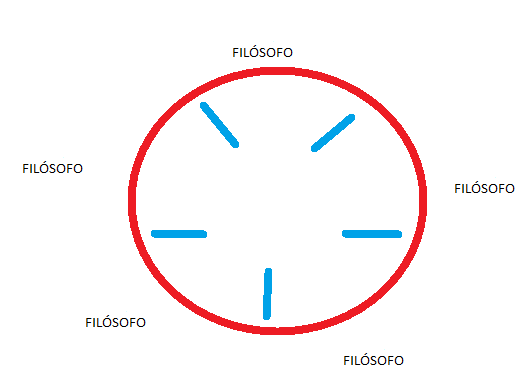
\includegraphics{Filosofos.png}
\caption{Esquema de los filósofos}\end{figure}


\subsection{Boceto de solución}
\label{textos/tema2:boceto-de-solucion}
\begin{Verbatim}[commandchars=\\\{\}]
\PYG{k+kn}{import} \PYG{n+nn}{java.util.Random}\PYG{o}{;}


\PYG{k+kd}{public} \PYG{k+kd}{class} \PYG{n+nc}{Filosofo}  \PYG{k+kd}{implements} \PYG{n}{Runnable}\PYG{o}{\PYGZob{}}
        \PYG{k+kd}{public} \PYG{k+kt}{void} \PYG{n+nf}{run}\PYG{o}{(}\PYG{o}{)}\PYG{o}{\PYGZob{}}
                \PYG{n}{String} \PYG{n}{miNombre}\PYG{o}{=}\PYG{n}{Thread}\PYG{o}{.}\PYG{n+na}{currentThread}\PYG{o}{(}\PYG{o}{)}\PYG{o}{.}\PYG{n+na}{getName}\PYG{o}{(}\PYG{o}{)}\PYG{o}{;}
                \PYG{n}{Random} \PYG{n}{generador}\PYG{o}{=}\PYG{k}{new} \PYG{n}{Random}\PYG{o}{(}\PYG{o}{)}\PYG{o}{;}
                \PYG{k}{while} \PYG{o}{(}\PYG{k+kc}{true}\PYG{o}{)}\PYG{o}{\PYGZob{}}
                        \PYG{c+cm}{/* Comer*/}
                        \PYG{c+cm}{/* Intentar coger palillos*/}
                        \PYG{c+cm}{/* Si los coge:*/}
                        \PYG{n}{System}\PYG{o}{.}\PYG{n+na}{out}\PYG{o}{.}\PYG{n+na}{println}\PYG{o}{(}\PYG{n}{miNombre}\PYG{o}{+}\PYG{l+s}{\PYGZdq{} comiendo...\PYGZdq{}}\PYG{o}{)}\PYG{o}{;}
                        \PYG{k+kt}{int} \PYG{n}{milisegs}\PYG{o}{=}\PYG{o}{(}\PYG{l+m+mi}{1}\PYG{o}{+}\PYG{n}{generador}\PYG{o}{.}\PYG{n+na}{nextInt}\PYG{o}{(}\PYG{l+m+mi}{5}\PYG{o}{)}\PYG{o}{)}\PYG{o}{*}\PYG{l+m+mi}{1000}\PYG{o}{;}
                        \PYG{n}{esperarTiempoAzar}\PYG{o}{(}\PYG{n}{miNombre}\PYG{o}{,} \PYG{n}{milisegs}\PYG{o}{)}\PYG{o}{;}
                        \PYG{c+cm}{/* Pensando...*/}
                        \PYG{c+c1}{//Recordemos soltar los palillos}
                        \PYG{n}{System}\PYG{o}{.}\PYG{n+na}{out}\PYG{o}{.}\PYG{n+na}{println}\PYG{o}{(}\PYG{n}{miNombre}\PYG{o}{+}\PYG{l+s}{\PYGZdq{}  pensando...\PYGZdq{}}\PYG{o}{)}\PYG{o}{;}                           \PYG{n}{milisegs}\PYG{o}{=}\PYG{o}{(}\PYG{l+m+mi}{1}\PYG{o}{+}\PYG{n}{generador}\PYG{o}{.}\PYG{n+na}{nextInt}\PYG{o}{(}\PYG{l+m+mi}{5}\PYG{o}{)}\PYG{o}{)}\PYG{o}{*}\PYG{l+m+mi}{1000}\PYG{o}{;}
                        \PYG{n}{esperarTiempoAzar}\PYG{o}{(}\PYG{n}{miNombre}\PYG{o}{,} \PYG{n}{milisegs}\PYG{o}{)}\PYG{o}{;}
                \PYG{o}{\PYGZcb{}}
        \PYG{o}{\PYGZcb{}}

\PYG{k+kd}{private} \PYG{k+kt}{void} \PYG{n+nf}{esperarTiempoAzar}\PYG{o}{(}\PYG{n}{String} \PYG{n}{miNombre}\PYG{o}{,} \PYG{k+kt}{int} \PYG{n}{milisegs}\PYG{o}{)} \PYG{o}{\PYGZob{}}
                \PYG{k}{try} \PYG{o}{\PYGZob{}}
                        \PYG{n}{Thread}\PYG{o}{.}\PYG{n+na}{sleep}\PYG{o}{(}\PYG{n}{milisegs}\PYG{o}{)}\PYG{o}{;}
                \PYG{o}{\PYGZcb{}} \PYG{k}{catch} \PYG{o}{(}\PYG{n}{InterruptedException} \PYG{n}{e}\PYG{o}{)} \PYG{o}{\PYGZob{}}
                        \PYG{n}{System}\PYG{o}{.}\PYG{n+na}{out}\PYG{o}{.}\PYG{n+na}{println}\PYG{o}{(}
                                        \PYG{n}{miNombre}\PYG{o}{+}\PYG{l+s}{\PYGZdq{} interrumpido!!. Saliendo...\PYGZdq{}}\PYG{o}{)}\PYG{o}{;}
                        \PYG{k}{return} \PYG{o}{;}
                \PYG{o}{\PYGZcb{}}
        \PYG{o}{\PYGZcb{}}
\PYG{o}{\PYGZcb{}}
\end{Verbatim}


\section{Solución completa al problema de los filósofos}
\label{textos/tema2:solucion-completa-al-problema-de-los-filosofos}

\subsection{Gestor de recursos compartidos (palillos)}
\label{textos/tema2:gestor-de-recursos-compartidos-palillos}
\begin{Verbatim}[commandchars=\\\{\}]
\PYG{k+kd}{public} \PYG{k+kd}{class} \PYG{n+nc}{GestorPalillos} \PYG{o}{\PYGZob{}}
        \PYG{c+cm}{/* False significa que no están cogidos*/}
        \PYG{k+kd}{private} \PYG{k+kt}{boolean}\PYG{o}{[}\PYG{o}{]} \PYG{n}{palillos}\PYG{o}{;}
        \PYG{k+kd}{public} \PYG{n+nf}{GestorPalillos}\PYG{o}{(}\PYG{k+kt}{int} \PYG{n}{num\PYGZus{}filosofos}\PYG{o}{)}\PYG{o}{\PYGZob{}}
                \PYG{n}{palillos}\PYG{o}{=}\PYG{k}{new} \PYG{k+kt}{boolean}\PYG{o}{[}\PYG{n}{num\PYGZus{}filosofos}\PYG{o}{]}\PYG{o}{;}
                \PYG{k}{for} \PYG{o}{(}\PYG{k+kt}{int} \PYG{n}{i}\PYG{o}{=}\PYG{l+m+mi}{0}\PYG{o}{;}\PYG{n}{i}\PYG{o}{\PYGZlt{}}\PYG{n}{palillos}\PYG{o}{.}\PYG{n+na}{length}\PYG{o}{;}\PYG{n}{i}\PYG{o}{+}\PYG{o}{+}\PYG{o}{)}\PYG{o}{\PYGZob{}}
                        \PYG{n}{palillos}\PYG{o}{[}\PYG{n}{i}\PYG{o}{]}\PYG{o}{=}\PYG{k+kc}{false}\PYG{o}{;}
                \PYG{o}{\PYGZcb{}}
        \PYG{o}{\PYGZcb{}}
        \PYG{k+kd}{public} \PYG{k+kd}{synchronized} \PYG{k+kt}{boolean}
                \PYG{n+nf}{sePuedenCogerAmbosPalillos}\PYG{o}{(}
                        \PYG{k+kt}{int} \PYG{n}{num1}\PYG{o}{,}\PYG{k+kt}{int} \PYG{n}{num2}\PYG{o}{)}\PYG{o}{\PYGZob{}}
                \PYG{k}{if} \PYG{o}{(} \PYG{o}{(}\PYG{n}{palillos}\PYG{o}{[}\PYG{n}{num1}\PYG{o}{]}\PYG{o}{=}\PYG{o}{=}\PYG{k+kc}{false}\PYG{o}{)} \PYG{o}{\PYGZam{}}\PYG{o}{\PYGZam{}}
                        \PYG{o}{(}\PYG{n}{palillos}\PYG{o}{[}\PYG{n}{num2}\PYG{o}{]}\PYG{o}{=}\PYG{o}{=}\PYG{k+kc}{false}\PYG{o}{)} \PYG{o}{)} \PYG{o}{\PYGZob{}}
                        \PYG{n}{palillos}\PYG{o}{[}\PYG{n}{num1}\PYG{o}{]}\PYG{o}{=}\PYG{k+kc}{true}\PYG{o}{;}
                        \PYG{n}{palillos}\PYG{o}{[}\PYG{n}{num2}\PYG{o}{]}\PYG{o}{=}\PYG{k+kc}{true}\PYG{o}{;}
                        \PYG{n}{System}\PYG{o}{.}\PYG{n+na}{out}\PYG{o}{.}\PYG{n+na}{println}\PYG{o}{(}
                                        \PYG{l+s}{\PYGZdq{}Alguien consiguio los palillos \PYGZdq{}}\PYG{o}{+}\PYG{n}{num1}\PYG{o}{+}\PYG{l+s}{\PYGZdq{} y \PYGZdq{}}\PYG{o}{+}\PYG{n}{num2}\PYG{o}{)}\PYG{o}{;}
                        \PYG{k}{return} \PYG{k+kc}{true}\PYG{o}{;}
                \PYG{o}{\PYGZcb{}}
                \PYG{k}{return} \PYG{k+kc}{false}\PYG{o}{;}
        \PYG{o}{\PYGZcb{}}
        \PYG{k+kd}{public} \PYG{k+kd}{synchronized} \PYG{k+kt}{void} \PYG{n+nf}{soltarPalillos}\PYG{o}{(}\PYG{k+kt}{int} \PYG{n}{num1}\PYG{o}{,} \PYG{k+kt}{int} \PYG{n}{num2}\PYG{o}{)}\PYG{o}{\PYGZob{}}
                \PYG{n}{palillos}\PYG{o}{[}\PYG{n}{num1}\PYG{o}{]}\PYG{o}{=}\PYG{k+kc}{false}\PYG{o}{;}
                \PYG{n}{palillos}\PYG{o}{[}\PYG{n}{num2}\PYG{o}{]}\PYG{o}{=}\PYG{k+kc}{false}\PYG{o}{;}
                \PYG{n}{System}\PYG{o}{.}\PYG{n+na}{out}\PYG{o}{.}\PYG{n+na}{println}\PYG{o}{(}
                                \PYG{l+s}{\PYGZdq{}Alguien liberó los palillos \PYGZdq{}}\PYG{o}{+}\PYG{n}{num1}\PYG{o}{+}\PYG{l+s}{\PYGZdq{} y \PYGZdq{}}\PYG{o}{+}\PYG{n}{num2}\PYG{o}{)}\PYG{o}{;}
        \PYG{o}{\PYGZcb{}}
\PYG{o}{\PYGZcb{}}
\end{Verbatim}


\subsection{Simulación de un filósofo}
\label{textos/tema2:simulacion-de-un-filosofo}
\begin{Verbatim}[commandchars=\\\{\}]
\PYG{k+kn}{import} \PYG{n+nn}{java.util.Random}\PYG{o}{;}
\PYG{k+kd}{public} \PYG{k+kd}{class} \PYG{n+nc}{Filosofo}  \PYG{k+kd}{implements} \PYG{n}{Runnable}\PYG{o}{\PYGZob{}}
        \PYG{k+kt}{int} \PYG{n}{num\PYGZus{}palillo\PYGZus{}izq}\PYG{o}{;}
        \PYG{k+kt}{int} \PYG{n}{num\PYGZus{}palillo\PYGZus{}der}\PYG{o}{;}
        \PYG{n}{GestorPalillos} \PYG{n}{gestorPalillos}\PYG{o}{;}
        \PYG{k+kd}{public} \PYG{n+nf}{Filosofo}\PYG{o}{(}\PYG{n}{GestorPalillos} \PYG{n}{gp}\PYG{o}{,}
                        \PYG{k+kt}{int} \PYG{n}{p\PYGZus{}izq}\PYG{o}{,} \PYG{k+kt}{int} \PYG{n}{p\PYGZus{}der}\PYG{o}{)}\PYG{o}{\PYGZob{}}
                \PYG{k}{this}\PYG{o}{.}\PYG{n+na}{gestorPalillos}\PYG{o}{=}\PYG{n}{gp}\PYG{o}{;}
                \PYG{k}{this}\PYG{o}{.}\PYG{n+na}{num\PYGZus{}palillo\PYGZus{}der}\PYG{o}{=}\PYG{n}{p\PYGZus{}der}\PYG{o}{;}
                \PYG{k}{this}\PYG{o}{.}\PYG{n+na}{num\PYGZus{}palillo\PYGZus{}izq}\PYG{o}{=}\PYG{n}{p\PYGZus{}izq}\PYG{o}{;}
        \PYG{o}{\PYGZcb{}}
        \PYG{k+kd}{public} \PYG{k+kt}{void} \PYG{n+nf}{run}\PYG{o}{(}\PYG{o}{)}\PYG{o}{\PYGZob{}}
                \PYG{n}{String} \PYG{n}{miNombre}\PYG{o}{=}\PYG{n}{Thread}\PYG{o}{.}\PYG{n+na}{currentThread}\PYG{o}{(}\PYG{o}{)}\PYG{o}{.}\PYG{n+na}{getName}\PYG{o}{(}\PYG{o}{)}\PYG{o}{;}
                \PYG{n}{Random} \PYG{n}{generador}\PYG{o}{=}\PYG{k}{new} \PYG{n}{Random}\PYG{o}{(}\PYG{o}{)}\PYG{o}{;}
                \PYG{k}{while} \PYG{o}{(}\PYG{k+kc}{true}\PYG{o}{)}\PYG{o}{\PYGZob{}}
                        \PYG{c+cm}{/* Comer*/}
                        \PYG{c+cm}{/* Intentar coger palillos*/}
                        \PYG{k}{while}\PYG{o}{(}\PYG{o}{!}\PYG{n}{gestorPalillos}\PYG{o}{.}\PYG{n+na}{sePuedenCogerAmbosPalillos}
                                        \PYG{o}{(}
                                                        \PYG{n}{num\PYGZus{}palillo\PYGZus{}izq}\PYG{o}{,} \PYG{n}{num\PYGZus{}palillo\PYGZus{}der}
                                        \PYG{o}{)}\PYG{o}{)}
                        \PYG{o}{\PYGZob{}}

                        \PYG{o}{\PYGZcb{}}
                        \PYG{c+cm}{/* Si los coge:*/}

                        \PYG{k+kt}{int} \PYG{n}{milisegs}\PYG{o}{=}\PYG{o}{(}\PYG{l+m+mi}{1}\PYG{o}{+}\PYG{n}{generador}\PYG{o}{.}\PYG{n+na}{nextInt}\PYG{o}{(}\PYG{l+m+mi}{5}\PYG{o}{)}\PYG{o}{)}\PYG{o}{*}\PYG{l+m+mi}{1000}\PYG{o}{;}
                        \PYG{n}{esperarTiempoAzar}\PYG{o}{(}\PYG{n}{miNombre}\PYG{o}{,} \PYG{n}{milisegs}\PYG{o}{)}\PYG{o}{;}
                        \PYG{c+cm}{/* Pensando...*/}
                        \PYG{c+c1}{//Recordemos soltar los palillos}
                        \PYG{n}{gestorPalillos}\PYG{o}{.}\PYG{n+na}{soltarPalillos}\PYG{o}{(}\PYG{n}{num\PYGZus{}palillo\PYGZus{}izq}\PYG{o}{,} \PYG{n}{num\PYGZus{}palillo\PYGZus{}der}\PYG{o}{)}\PYG{o}{;}

                        \PYG{n}{milisegs}\PYG{o}{=}\PYG{o}{(}\PYG{l+m+mi}{1}\PYG{o}{+}\PYG{n}{generador}\PYG{o}{.}\PYG{n+na}{nextInt}\PYG{o}{(}\PYG{l+m+mi}{5}\PYG{o}{)}\PYG{o}{)}\PYG{o}{*}\PYG{l+m+mi}{1000}\PYG{o}{;}
                        \PYG{n}{esperarTiempoAzar}\PYG{o}{(}\PYG{n}{miNombre}\PYG{o}{,} \PYG{n}{milisegs}\PYG{o}{)}\PYG{o}{;}
                \PYG{o}{\PYGZcb{}}
        \PYG{o}{\PYGZcb{}}

\PYG{k+kd}{private} \PYG{k+kt}{void} \PYG{n+nf}{esperarTiempoAzar}\PYG{o}{(}\PYG{n}{String} \PYG{n}{miNombre}\PYG{o}{,} \PYG{k+kt}{int} \PYG{n}{milisegs}\PYG{o}{)} \PYG{o}{\PYGZob{}}
                \PYG{k}{try} \PYG{o}{\PYGZob{}}
                        \PYG{n}{Thread}\PYG{o}{.}\PYG{n+na}{sleep}\PYG{o}{(}\PYG{n}{milisegs}\PYG{o}{)}\PYG{o}{;}
                \PYG{o}{\PYGZcb{}} \PYG{k}{catch} \PYG{o}{(}\PYG{n}{InterruptedException} \PYG{n}{e}\PYG{o}{)} \PYG{o}{\PYGZob{}}
                        \PYG{n}{System}\PYG{o}{.}\PYG{n+na}{out}\PYG{o}{.}\PYG{n+na}{println}\PYG{o}{(}
                                        \PYG{n}{miNombre}\PYG{o}{+}\PYG{l+s}{\PYGZdq{} interrumpido!!. Saliendo...\PYGZdq{}}\PYG{o}{)}\PYG{o}{;}
                        \PYG{k}{return} \PYG{o}{;}
                \PYG{o}{\PYGZcb{}}
        \PYG{o}{\PYGZcb{}}
\PYG{o}{\PYGZcb{}}
\end{Verbatim}


\subsection{Lanzador de hilos}
\label{textos/tema2:lanzador-de-hilos}
\begin{Verbatim}[commandchars=\\\{\}]
\PYG{k+kd}{public} \PYG{k+kd}{class} \PYG{n+nc}{LanzadorFilosofos} \PYG{o}{\PYGZob{}}
        \PYG{k+kd}{public} \PYG{k+kd}{static} \PYG{k+kt}{void} \PYG{n+nf}{main}\PYG{o}{(}\PYG{n}{String}\PYG{o}{[}\PYG{o}{]} \PYG{n}{args}\PYG{o}{)} \PYG{o}{\PYGZob{}}
                \PYG{k+kt}{int} \PYG{n}{MAX\PYGZus{}FILOSOFOS}\PYG{o}{=}\PYG{l+m+mi}{5}\PYG{o}{;}
                \PYG{n}{Filosofo}\PYG{o}{[}\PYG{o}{]} \PYG{n}{filosofos}\PYG{o}{=}\PYG{k}{new} \PYG{n}{Filosofo}\PYG{o}{[}\PYG{n}{MAX\PYGZus{}FILOSOFOS}\PYG{o}{]}\PYG{o}{;}
                \PYG{n}{Thread}\PYG{o}{[}\PYG{o}{]} \PYG{n}{hilosAsociados}\PYG{o}{=}\PYG{k}{new} \PYG{n}{Thread}\PYG{o}{[}\PYG{n}{MAX\PYGZus{}FILOSOFOS}\PYG{o}{]}\PYG{o}{;}
                \PYG{n}{GestorPalillos} \PYG{n}{gestorCompartido}\PYG{o}{=}
                                \PYG{k}{new} \PYG{n+nf}{GestorPalillos}\PYG{o}{(}\PYG{n}{MAX\PYGZus{}FILOSOFOS}\PYG{o}{)}\PYG{o}{;}
                \PYG{k}{for} \PYG{o}{(}\PYG{k+kt}{int} \PYG{n}{i}\PYG{o}{=}\PYG{l+m+mi}{0}\PYG{o}{;} \PYG{n}{i}\PYG{o}{\PYGZlt{}}\PYG{n}{MAX\PYGZus{}FILOSOFOS}\PYG{o}{;} \PYG{n}{i}\PYG{o}{+}\PYG{o}{+}\PYG{o}{)}\PYG{o}{\PYGZob{}}
                        \PYG{k}{if} \PYG{o}{(}\PYG{n}{i}\PYG{o}{=}\PYG{o}{=}\PYG{l+m+mi}{0}\PYG{o}{)}\PYG{o}{\PYGZob{}}
                                \PYG{n}{filosofos}\PYG{o}{[}\PYG{n}{i}\PYG{o}{]}\PYG{o}{=}\PYG{k}{new} \PYG{n}{Filosofo}\PYG{o}{(}
                                                \PYG{n}{gestorCompartido}\PYG{o}{,} \PYG{n}{i}\PYG{o}{,}\PYG{n}{MAX\PYGZus{}FILOSOFOS}\PYG{o}{\PYGZhy{}}\PYG{l+m+mi}{1}\PYG{o}{)}\PYG{o}{;}
                        \PYG{o}{\PYGZcb{}}
                        \PYG{k}{else} \PYG{o}{\PYGZob{}}
                                \PYG{n}{filosofos}\PYG{o}{[}\PYG{n}{i}\PYG{o}{]}\PYG{o}{=}\PYG{k}{new} \PYG{n}{Filosofo}\PYG{o}{(}
                                                \PYG{n}{gestorCompartido}\PYG{o}{,} \PYG{n}{i}\PYG{o}{,} \PYG{n}{i}\PYG{o}{\PYGZhy{}}\PYG{l+m+mi}{1}\PYG{o}{)}\PYG{o}{;}
                        \PYG{o}{\PYGZcb{}}
                        \PYG{n}{Thread} \PYG{n}{hilo}\PYG{o}{=}\PYG{k}{new} \PYG{n}{Thread}\PYG{o}{(}\PYG{n}{filosofos}\PYG{o}{[}\PYG{n}{i}\PYG{o}{]}\PYG{o}{)}\PYG{o}{;}
                        \PYG{n}{hilo}\PYG{o}{.}\PYG{n+na}{setName}\PYG{o}{(}\PYG{l+s}{\PYGZdq{}Filosofo \PYGZdq{}}\PYG{o}{+}\PYG{n}{i}\PYG{o}{)}\PYG{o}{;}
                        \PYG{n}{hilosAsociados}\PYG{o}{[}\PYG{n}{i}\PYG{o}{]}\PYG{o}{=}\PYG{n}{hilo}\PYG{o}{;}
                        \PYG{n}{hilo}\PYG{o}{.}\PYG{n+na}{start}\PYG{o}{(}\PYG{o}{)}\PYG{o}{;}
                \PYG{o}{\PYGZcb{}}
                \PYG{c+cm}{/* Un poco inútil*/}
                \PYG{k}{for} \PYG{o}{(}\PYG{k+kt}{int} \PYG{n}{i}\PYG{o}{=}\PYG{l+m+mi}{0}\PYG{o}{;} \PYG{n}{i}\PYG{o}{\PYGZlt{}}\PYG{n}{MAX\PYGZus{}FILOSOFOS}\PYG{o}{;}\PYG{n}{i}\PYG{o}{+}\PYG{o}{+}\PYG{o}{)}\PYG{o}{\PYGZob{}}
                        \PYG{k}{try} \PYG{o}{\PYGZob{}}
                                \PYG{n}{hilosAsociados}\PYG{o}{[}\PYG{n}{i}\PYG{o}{]}\PYG{o}{.}\PYG{n+na}{join}\PYG{o}{(}\PYG{o}{)}\PYG{o}{;}
                        \PYG{o}{\PYGZcb{}} \PYG{k}{catch} \PYG{o}{(}\PYG{n}{InterruptedException} \PYG{n}{e}\PYG{o}{)} \PYG{o}{\PYGZob{}}
                                \PYG{c+c1}{// TODO Auto\PYGZhy{}generated catch block}
                                \PYG{n}{e}\PYG{o}{.}\PYG{n+na}{printStackTrace}\PYG{o}{(}\PYG{o}{)}\PYG{o}{;}
                        \PYG{o}{\PYGZcb{}}
                \PYG{o}{\PYGZcb{}}
        \PYG{o}{\PYGZcb{}}
\PYG{o}{\PYGZcb{}}
\end{Verbatim}


\section{Documentación.}
\label{textos/tema2:documentacion}

\section{Depuración.}
\label{textos/tema2:depuracion}

\chapter{Programación de comunicaciones en red}
\label{textos/tema3:programacion-de-comunicaciones-en-red}\label{textos/tema3::doc}

\section{Comunicación entre aplicaciones.}
\label{textos/tema3:comunicacion-entre-aplicaciones}

\section{Roles cliente y servidor.}
\label{textos/tema3:roles-cliente-y-servidor}

\section{Elementos de programación de aplicaciones en red. Librerías.}
\label{textos/tema3:elementos-de-programacion-de-aplicaciones-en-red-librerias}

\section{Funciones y objetos de las librerías.}
\label{textos/tema3:funciones-y-objetos-de-las-librerias}

\section{Sockets.}
\label{textos/tema3:sockets}

\section{Tipos de sockets. Características.}
\label{textos/tema3:tipos-de-sockets-caracteristicas}

\section{Creación de sockets.}
\label{textos/tema3:creacion-de-sockets}

\section{Enlazado y establecimiento de conexiones.}
\label{textos/tema3:enlazado-y-establecimiento-de-conexiones}

\section{Utilización de sockets para la transmisión y recepción de información.}
\label{textos/tema3:utilizacion-de-sockets-para-la-transmision-y-recepcion-de-informacion}

\section{Programación de aplicaciones cliente y servidor.}
\label{textos/tema3:programacion-de-aplicaciones-cliente-y-servidor}

\section{Utilización de hilos en la programación de aplicaciones en red.}
\label{textos/tema3:utilizacion-de-hilos-en-la-programacion-de-aplicaciones-en-red}

\section{Depuración.}
\label{textos/tema3:depuracion}

\chapter{Generación de servicios en red}
\label{textos/tema4::doc}\label{textos/tema4:generacion-de-servicios-en-red}

\section{Protocolos estándar de comunicación en red a nivel de aplicación}
\label{textos/tema4:protocolos-estandar-de-comunicacion-en-red-a-nivel-de-aplicacion}

\subsection{Telnet}
\label{textos/tema4:telnet}

\subsection{FTP}
\label{textos/tema4:ftp}

\subsection{HTTP}
\label{textos/tema4:http}

\subsection{POP3}
\label{textos/tema4:pop3}

\subsection{SMTP}
\label{textos/tema4:smtp}

\section{Librerías de clases y componentes.}
\label{textos/tema4:librerias-de-clases-y-componentes}

\section{Utilización de objetos predefinidos.}
\label{textos/tema4:utilizacion-de-objetos-predefinidos}

\section{Propiedades de los objetos predefinidos.}
\label{textos/tema4:propiedades-de-los-objetos-predefinidos}

\section{Métodos y eventos de los objetos predefinidos.}
\label{textos/tema4:metodos-y-eventos-de-los-objetos-predefinidos}

\section{Establecimiento y finalización de conexiones.}
\label{textos/tema4:establecimiento-y-finalizacion-de-conexiones}

\section{Transmisión de información.}
\label{textos/tema4:transmision-de-informacion}

\section{Programación de aplicaciones cliente.}
\label{textos/tema4:programacion-de-aplicaciones-cliente}

\section{Programación de servidores.}
\label{textos/tema4:programacion-de-servidores}

\section{Implementación de comunicaciones simultáneas.}
\label{textos/tema4:implementacion-de-comunicaciones-simultaneas}

\section{Documentación.}
\label{textos/tema4:documentacion}

\section{Depuración.}
\label{textos/tema4:depuracion}

\section{Monitorización de tiempos de respuesta.}
\label{textos/tema4:monitorizacion-de-tiempos-de-respuesta}

\chapter{Utilización de técnicas de programación segura}
\label{textos/tema5::doc}\label{textos/tema5:utilizacion-de-tecnicas-de-programacion-segura}

\section{Prácticas de programación segura.}
\label{textos/tema5:practicas-de-programacion-segura}

\section{Criptografía de clave pública y clave privada.}
\label{textos/tema5:criptografia-de-clave-publica-y-clave-privada}

\section{Principales aplicaciones de la criptografía.}
\label{textos/tema5:principales-aplicaciones-de-la-criptografia}

\section{Protocolos criptográficos.}
\label{textos/tema5:protocolos-criptograficos}

\section{Política de seguridad.}
\label{textos/tema5:politica-de-seguridad}

\section{Programación de mecanismos de control de acceso.}
\label{textos/tema5:programacion-de-mecanismos-de-control-de-acceso}

\section{Encriptación de información.}
\label{textos/tema5:encriptacion-de-informacion}

\section{Protocolos seguros de comunicaciones.}
\label{textos/tema5:protocolos-seguros-de-comunicaciones}

\section{Programación de aplicaciones con comunicaciones seguras.}
\label{textos/tema5:programacion-de-aplicaciones-con-comunicaciones-seguras}

\section{Pruebas y depuración.}
\label{textos/tema5:pruebas-y-depuracion}


\renewcommand{\indexname}{Índice}
\printindex
\end{document}
